\documentclass[12pt,reqno,twoside]{amsbook}
\usepackage{preamble}

% References File(s)
\addbibresource{references.bib}

% Change these values if the titles in your list of figures/tables intersect with the index numbers.
% =====================================================================
\lofskip{6pc} % Space between Figure index and title in  List of Figures
\lotskip{6pc} % Space between Table index and title in the List of Tables
% =====================================================================

% =====================================================================
%                               INFORMATION
% =====================================================================

% Title of the Dissertation
\title{A Cross-Layer SDN Orchestration Architecture for Stateful Edge Services}

% Author (Full Name)
\author{Pedro Ojo Oriakhi}

% Program (Name of Degree)
\program{Master's in Telecommunications and Computer Engineering}

% Department(s)
\department{Department of Information Science and Technology}

% Supervisors 
% ======================================================================
\supervisor
{Ph.D. Professor José Moura, Assistant Professor}
{Iscte - Instituto Universitário de Lisboa}

\supervisor
{Ph.D. Professor Pedro Ramos, Assistant Professor}
{Iscte - Instituto Universitário de Lisboa}

% ======================================================================

% Submission Date (Month, Year)
\date{Month}{Year}

% Acknowledgements -- Optional if no grants or fundings need to be listed.
\acknowledgements{
    Write here your acknowledgements and, if applicable, any grants or sources of funding.
}

% Dedication -- Optional
\dedication{
    Write here your dedication.
}

% Acronyms -- Optional, but you should use it if you use acronyms in your text!
%
% You can define as many acronyms as you want, like this:
%   \acro{TIAA}{This Is An Acronym}
% You can reference an acronym as-is inline using e.g. \ac{TIAA}.
% If you need to reference a pluralised acronym, instead use \acp.
\acronyms{
    \acro{SDN}{Software-Defined Networking}
    \acro{WSM}{Weighted Sum Model}
    \acro{VIP}{Virtual IP}
    \acro{OVS}{Open vSwitch}
    \acro{HPA}{Horizontal Pod Autoscaler}
    \acro{MEC}{Multi-Access Edge Computing}
    \acro{ZMQ}{ZeroMQ}
    \acro{RTT}{Round-Trip Time}
    \acro{RSS}{Resident Set Size}
    \acro{DSRM}{Design Science Research Methodology}
}
% =====================================================================










% =====================================================================
%                           RESUMO + ABSTRACT
% =====================================================================
% Resumo, em Português
% Abstract
\abstract{
    Write here the abstract in English. There is a 250 word limit.
}{
    Keywords; separated; by; semicolons
}
% =====================================================================

% =====================================================================
%                               MAIN BODY
% =====================================================================
\begin{document}

\chapter{Introduction}\label{ch:introduction}
Studies have shown that edge web services encompassing routing, monitoring and auto-scaling
can suffer from coordination delays that arise from the independent control loops through
which each module operates. This accumulation of handoff delays
between components degrades orchestration efficiency and reliability which can
potentially reduce service quality.

 In this chapter the context, motivation and problem statement are explained in 
\ref{sec:context_motivation} with the objectives presented in \ref{sec:objectives}. 
The research questions that emerged are available in \ref{sec:research_questions}. 
The methodology used to develop the thesis is detailed in \ref{sec:research_methodology},
the main contributions in \ref{sec:contributions} and finally the outlining of the rest of the 6 
chapters of the thesis are presented in \ref{sec:document_structure}.

\section{Context, Motivation, and Problem Statement}\label{sec:context_motivation}
In the year 2025 global internet traffic surpassed 7 exabytes 
(1 exabyte = 1 000 000 000 gigabytes), this 
corresponds to a more than double increase in the amount of internet traffic
generated since 2020 across fixed and mobile networks, this is represented in Figure 1.1.
\parencite{ITU2025InternetTraffic}.

\begin{figure}[H]
    \centering
    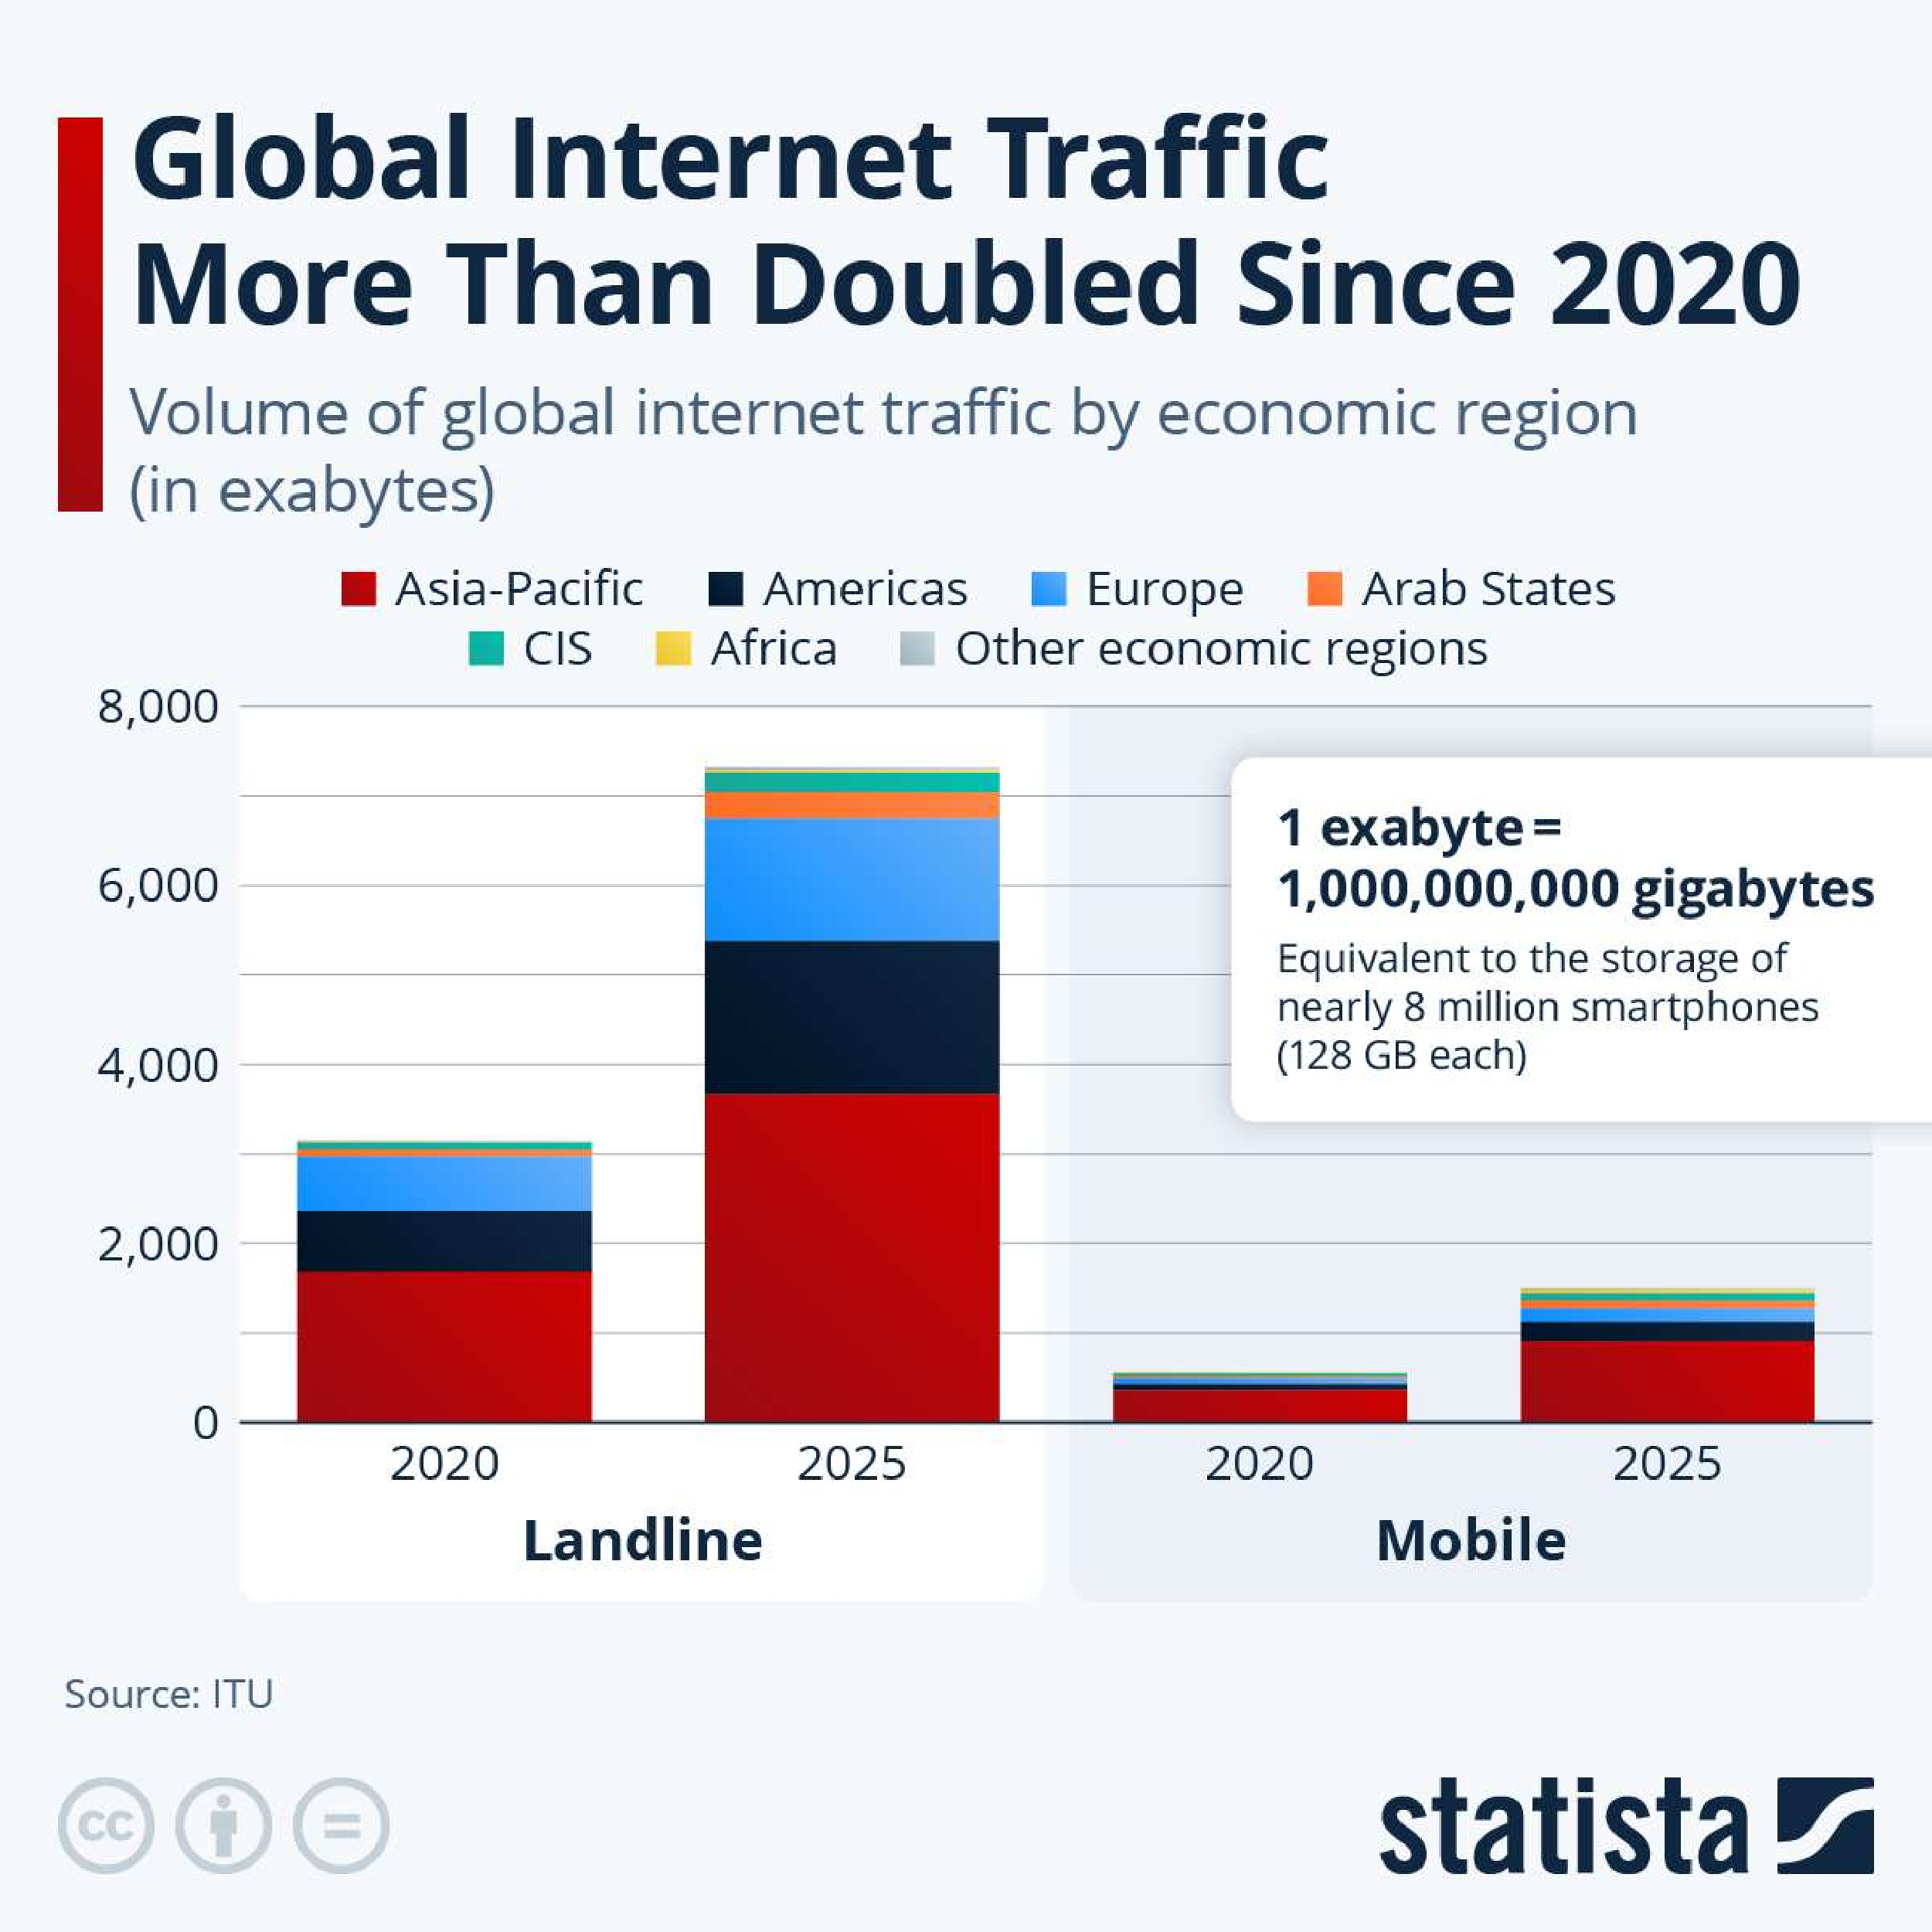
\includegraphics[width=0.4\textwidth]{images/global-internet-traffic-over-the-years.pdf}
    \caption{Global internet traffic between 2020 and 2025. Source: Statista, based on ITU data~\parencite{ITU2025InternetTraffic}.}
    \label{fig:internet_traffic}
\end{figure}

    This growth has been driven by many technological advancements some of which, 
have in turn galvanized the emergence of real-time interactive and data-intensive
applications among others. Examples include web streaming and cloud gaming, 
which are both services where users expect sub-second latency and high resolution
multimedia, highlighting the need for fast and capable data processing. These are just
a few examples that demonstrate the demand of infrastructure that is able to deliver
performance with high availability and reliability at global scale, in other words
regardless of where the end users are located.

Cloud computing is and has been the \parencite{Gurung2026CloudRevolutionTracingOriginsRise}
backbone that enables these applications to operate at a global scale. 
It offers automatic scaling, both horizontally and vertically,
a pay-per-use model and among other aspects, 
\parencite{Gurung2026CloudRevolutionTracingOriginsRise} a globally distributed offering
and availability that has established it as
the foundational layer that supports modern applications and services. 

    Yet, in parallel, a growing share of internet traffic now originates from
mobile devices, which have become the main gateway to internet access
\parencite{Gaudiaut2026MobileTrafficShare}. Much of this access is
therefore generated and consumed at the network edge, far from
centralised cloud data centres. As presented in 
\parencite{Cao2020OverviewEdgeComputingResearch},
\parencite{Satyanarayanan2017EmergenceEdgeComputing} edge computing brings
the computational resources to the network edge therefore closer to the
end-users, allowing for much lower latency in delivering services
and applications to users by leveraging its geo-distributed nature. 
Beyond lower latency, edge computing's inherent
geo-distributed servers dispersed geographically and close to users relieves bandwidth
pressure on the core network, since data can be processed and stored locally,
at the edge, for quicker responses, only a subset of it is sent to the cloud
\parencite{Cao2020OverviewEdgeComputingResearch},
freeing up backbone available bandwidth. 

    Despite these advantages, this geographical distribution also translates into
less capacity per location and greater complexity in managing the distributed
edge servers. As Satyanarayanan puts it, \enquote{the dispersion inherent in
edge computing raises the complexity of management considerably}
\parencite{Satyanarayanan2017EmergenceEdgeComputing}. This management complexity stems
from the dispersion of the edge servers across many sites,
aggravated by considerable variation in user demand over time and by the
heterogeneous resource requirements of the requests served. Luo et al. further
highlight that, without efficient resource scheduling, this distributed nature
leads to resource waste
\parencite{Luo2021ResourceSchedulingEdgeComputingSurvey}. Resource
management therefore becomes increasingly important, since the limited
capacity of each location must be adjusted over time to suit the constant
fluctuation of user demand.

    The resource management problem gains more relevance when the services
themselves are stateful. Unlike stateless microservices, which can be
replicated freely and absorb traffic immediately, stateful services in a
geo-distributed edge deployment depend on data co-located with compute:
a content item ingested at one site is served from the database of that
site. In distributed deployments, such data is routinely replicated
across sites for locality and robustness, but replication is neither
instantaneous nor free: a request reaching a server whose local copy is
still synchronising must wait for it to catch up, and maintaining copies
consumes storage and replication bandwidth
\parencite{Breitbach2019ContextAwareDataTaskPlacement},
\parencite{Nicolaescu2021StoreEdgeNetworkedDataSEND},
\parencite{Pelle2022CostLatencyEdgePlatform}.

    Scale-out alone does not guarantee usable capacity: the orchestration
system must detect when data must be brought closer, deliver that
information to the decision point, provision the right kind of capacity,
and redirect traffic to it, and each of these steps introduces delay that
worsens resource orchestration and can, in turn, lead to user service
quality degradation.

    This sequence forms what this dissertation calls the demand-to-capacity
chain: the default path that an orchestration system must traverse to convert
a change in overall user demand into capacity that serves that demand. A demand
shift is first observed by monitoring and telemetry, which deliver the
evidence to a decision point; the decision point selects a capacity action,
such as scaling compute or scaling storage; the action provisions the new
capacity; the new capacity attains a readiness state and is admitted
to traffic, which is the point at which it becomes usable. The chain is therefore a
timeline through the orchestration system,
and certain steps are separated from the next by an interface at which delay or
loss of evidence can accumulate.\footnote{Throughout this dissertation, the
\emph{demand-to-capacity chain} denotes the full timeline from a demand
shift to usable capacity; an \emph{interface} is a boundary between two
steps of the chain at which two functions meet; a \emph{handoff delay} is
the latency added at an interface when the functions on either side run
under independent control loops; and the \emph{coordination gap} is the
accumulated effect of these handoff delays along the chain.} Three of these
interfaces, more specifically how demand evidence reaches the decision, which capacity
action the decision selects, and when a ready backend is admitted to
traffic are the subject of this thesis. Figure~\ref{fig:demand_capacity_chain}
illustrates the chain.

\begin{figure}[H]
    \centering
    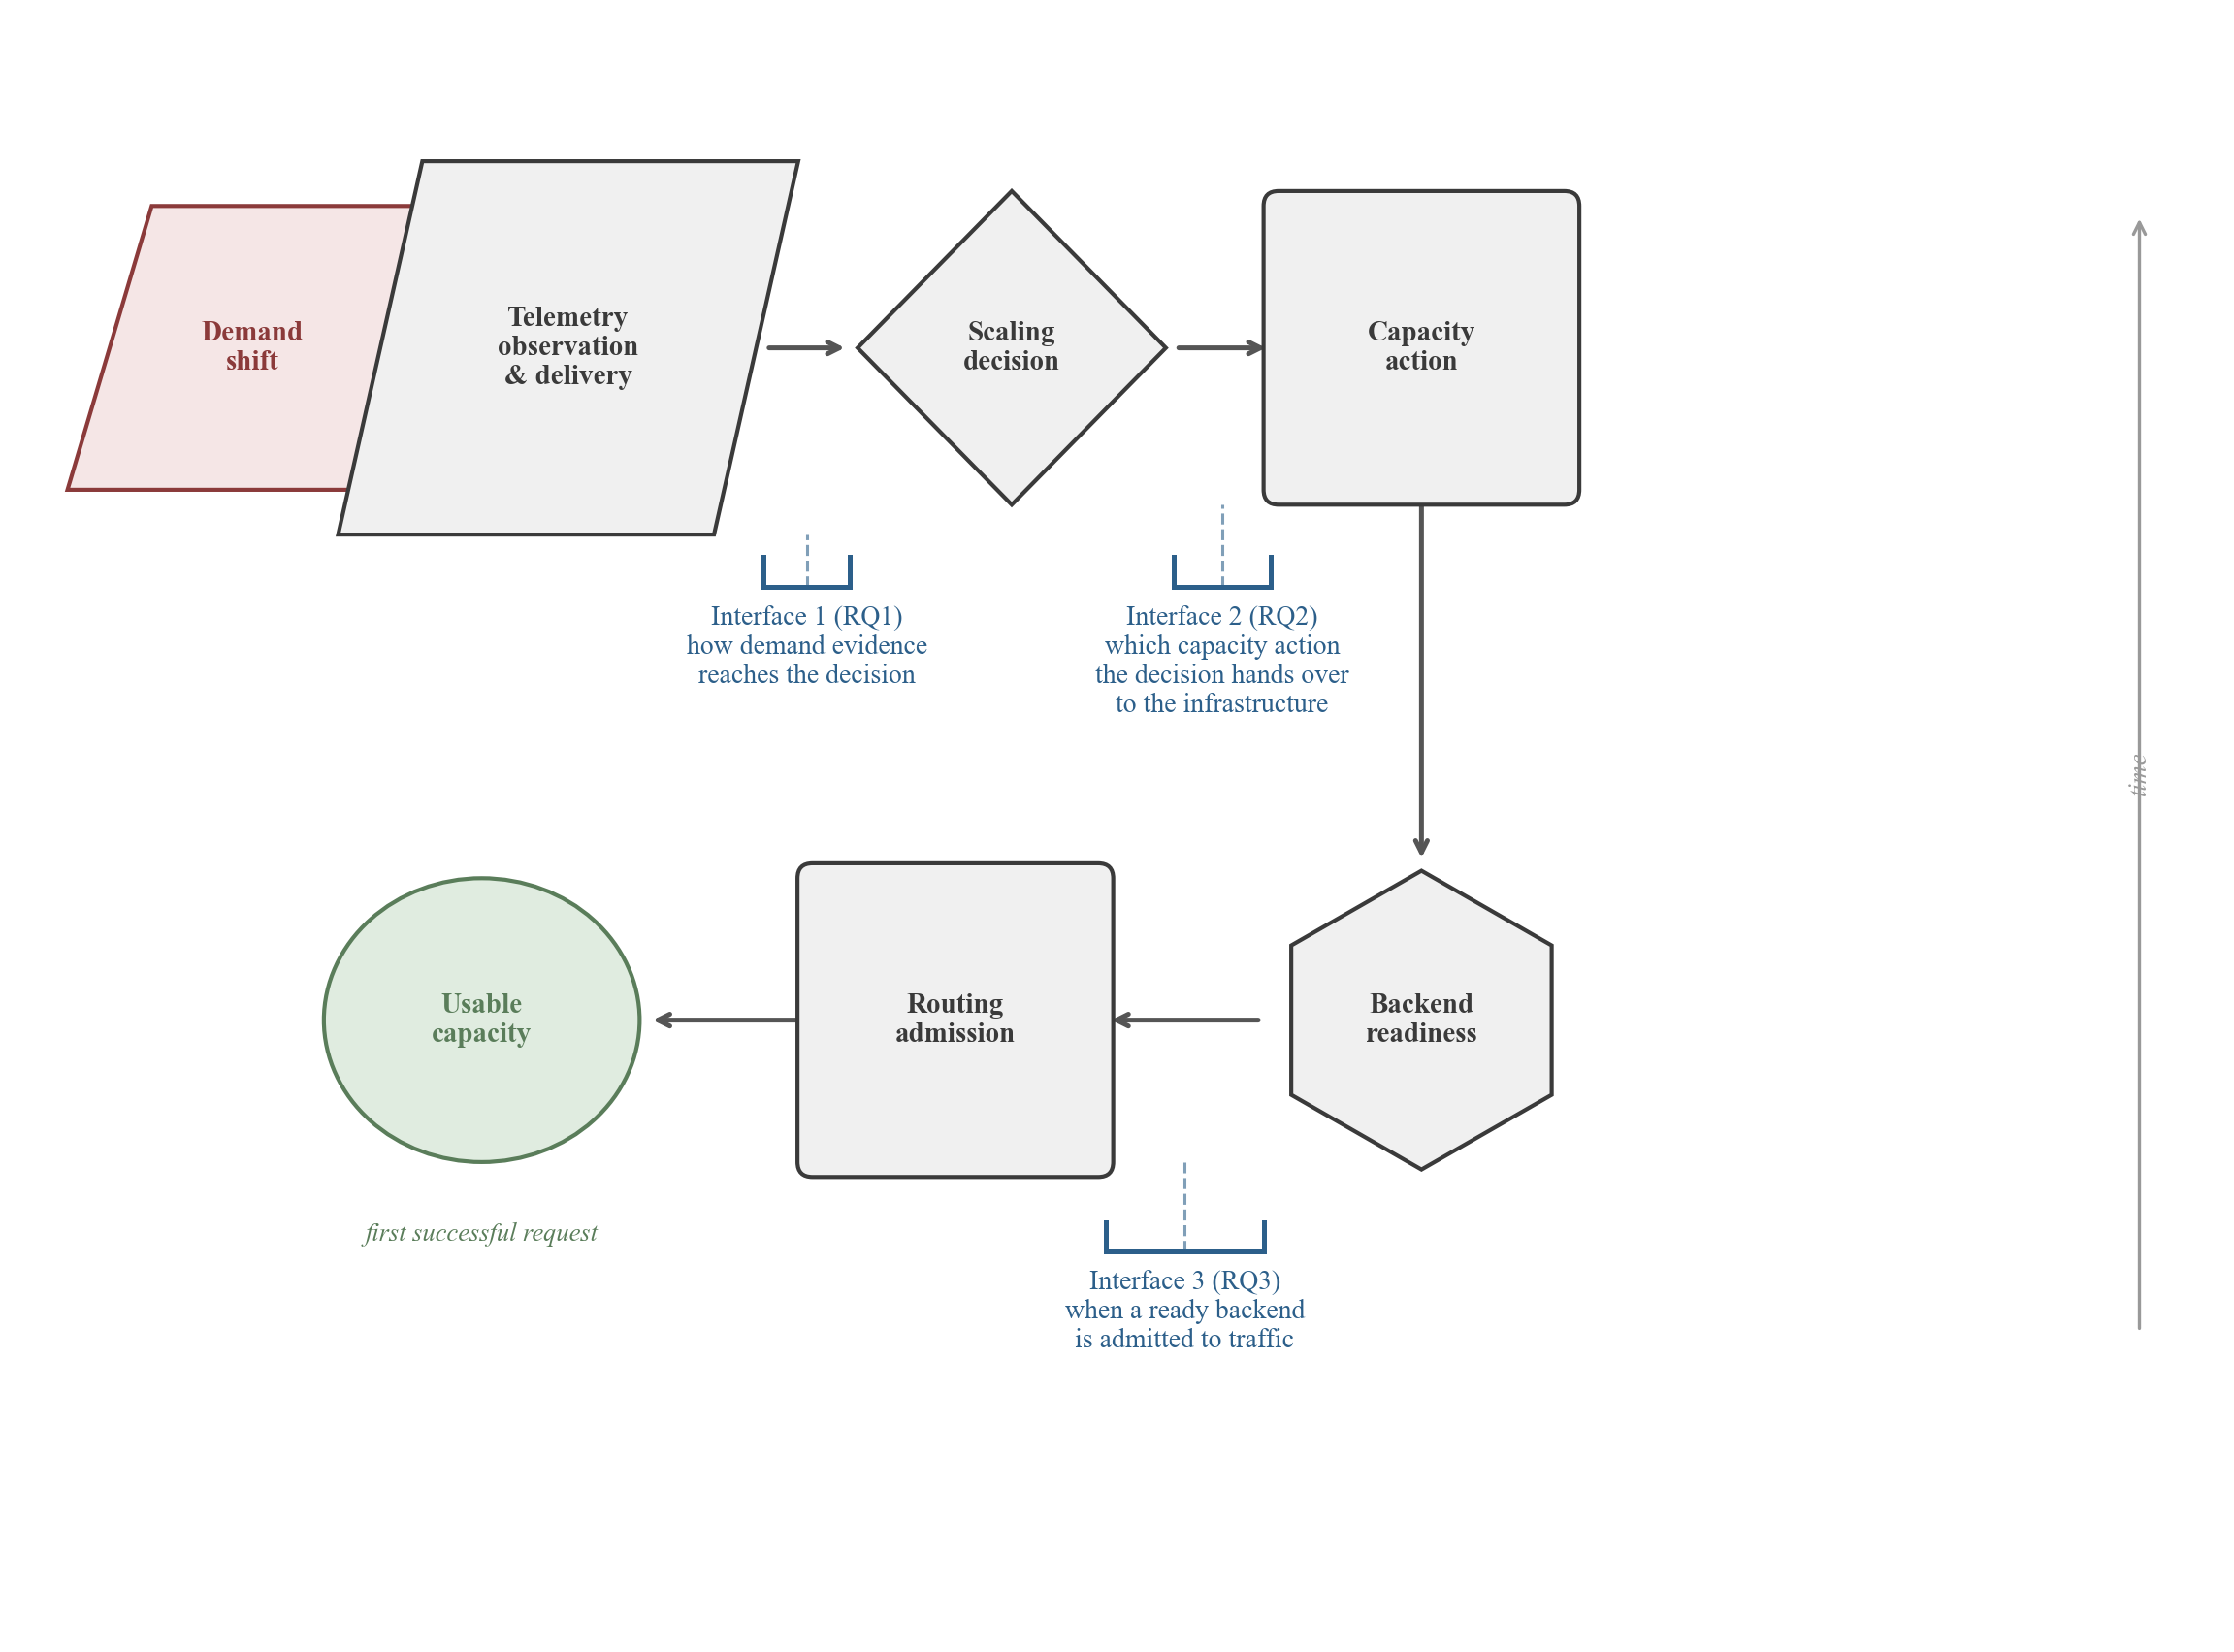
\includegraphics[width=0.9\textwidth]{images/demand_to_capacity_chain_v2.png}
    \caption{The demand-to-capacity chain: from a demand shift to usable
    capacity, with the three interfaces studied in this dissertation
    highlighted.}
    \label{fig:demand_capacity_chain}
\end{figure}

    The steps described above must be coordinated under the time pressure of
an ongoing demand shift. In practice, however, they are performed by
separate components: a monitoring system collects metrics, an
auto-scaler provisions capacity, and a load balancer redirects traffic,
each running under its own control loop. The information needed to
respond to demand must therefore cross from one component to the next,
and the delays accumulated at these handoffs determine how quickly newly
provisioned capacity can actually serve traffic. In the reviewed literature,
these handoffs are acknowledged in passing but never isolated or
varied as an independent variable
\parencite{Qu2018AutoScalingWebApplicationsClouds,Llorens2021SDNBasedHorizontalAutoScalingLoadBalancing}.
This thesis investigates them directly through two peer \ac{SDN}
controllers, one per network domain. Within each controller process,
telemetry consumption, scaling decisions, and traffic routing are co-located.
Telemetry production and aggregation remain external to the controller, making
the delivery of aggregated demand evidence an explicit and configurable
interface. Together with explicit lifecycle hooks for capacity action and
traffic admission, this arrangement allows each selected interface to be
measured under controlled conditions.

    Along this chain, three interfaces are studied in a stateful service
deployed across two geo-distributed sites: how demand evidence is
delivered to the controller (telemetry delivery semantics), which
capacity action the controller selects in response to the observed
bottleneck (compute or storage scale-out), and when ready capacity is
admitted to traffic (readiness admission).

    The thesis does not claim that this SDN-based architecture is
superior to existing orchestration platforms such as Kubernetes or NFV
MANO, nor that the platform mechanisms generalise
beyond the tested infrastructure; it claims only that these three
interfaces are measurable and, within the reviewed literature, not
previously characterised in isolation, and that varying each
independently reveals which dimensions matter and under what
conditions.

\section{Objectives}\label{sec:objectives}
The main objective of this thesis is to study the coordination gaps that
arise between independent modules with their own control loops and to
contribute to more efficient resource orchestration for stateful edge
services, by characterising a specific and less examined part of this
problem: the handoff delays that accumulate at the interfaces between
telemetry delivery, capacity action selection, and traffic admission
under varying demand shifts. The investigation rests on the idea that
co-locating telemetry consumption, scaling decisions, and routing within each
controller process keeps their controller-side coordination in-process while
retaining telemetry delivery as an explicit, configurable boundary. Along with
explicit lifecycle hooks for scaling and admission, this arrangement exposes
the selected interfaces to direct measurement. When one selected interface is
varied while the other interfaces and the surrounding platform are held
constant, its contribution to the demand-to-capacity timeline can be measured,
forming the basis of the experimental design.

    Because the co-located components are coupled,
making each interface independently variable is itself a deliberate
design of the platform, and that allows its impact to be measured not
only on the time from demand to usable capacity but also on service
quality, on how load is distributed across resources, and on how
flexibly the service responds to demand variation.

\section{Research Questions}\label{sec:research_questions}
This thesis seeks to answer the following three research questions:

\begin{itemize}
    \item \textbf{RQ1} -- How do verified event-preserving, delayed event-preserving,
    and latest-state telemetry delivery semantics affect overload observability,
    scaling response, and transient service quality in a stateful edge service?

    \item \textbf{RQ2} -- Under compute-bound and data-access-bound demand,
    how does bottleneck-aware scale-out, compared
    with fixed single-tier policies, affect
    targeted-tier relief, service recovery, and resource use?

    \item \textbf{RQ3} -- For newly provisioned compute backends satisfying an
    identical servability criterion, how do lifecycle-driven and periodic
    readiness-admission mechanisms affect the time from verified readiness to
    routable and usable capacity?
\end{itemize}

\section{Research Methodology}\label{sec:research_methodology}
The work presented in this dissertation follows the Design Science Research
(DSR) methodology \parencite{Hevner2004DesignScienceInformationSystemsResearch1},
\parencite{vomBrocke2020IntroductionDesignScienceResearch}
proposed in \parencite{Peffers2007DesignScienceResearchMethodologyInformation},
and demonstrated in Figure~\ref{fig:design_science_research_methodology}.

\begin{figure}[H]
    \centering
    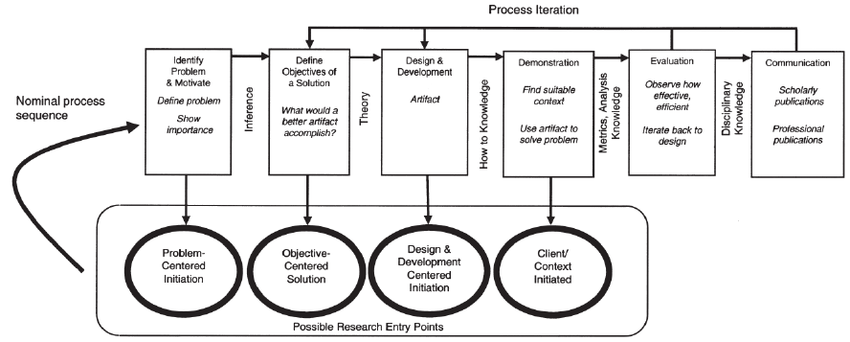
\includegraphics[width=0.8\textwidth]{images/Design Science Research process model.png}
    \caption{Design Science Research Methodology}
    \label{fig:design_science_research_methodology}    
\end{figure}

    Design science produces and evaluates purposeful artefacts that address certain
real-world problems, the research contribution lies in the knowledge generated
by designing the artefact and evaluating it against defined objectives. The \ac{DSRM} 
organises the research effort into six activities: problem
identification and motivation, definition of the objectives of a solution,
design and development, demonstration, evaluation, and communication.

    This dissertation follows a problem-centred approach where the problem motivates
the research and is defined as the coordination delays that accumulate between independently
operating control loops in edge orchestration of services, which is justified by the state of the art reviewed
in \ref{ch:literature_review}. The six activities unfolded as follows.

\begin{enumerate}
\item \textbf{Problem identification and motivation.} Edge services whose
monitoring, routing and scaling modules operate as independent components
accumulate handoff delays between control loops, degrading orchestration
efficiency. The problem is introduced in
\ref{sec:context_motivation}, and the review of the state of the art in
\ref{ch:literature_review} establishes both that these functions are typically
studied in isolation and that co-located architectures with independently
configurable interfaces are less commonly present in the reviewed literature, which
motivates and delimits the problem.

\item \textbf{Objectives of a solution.} As defined in \ref{sec:objectives},
the solution is an experimental platform, not a novel algorithm, whose
purpose is to make the interfaces of the demand-to-capacity chain
measurable, so that their contribution to resource orchestration can be
evaluated through measurement and better understood.

\item \textbf{Design and development.} The artefact is the co-located platform
described in \ref{ch:system_architecture} and \ref{ch:implementation}: two peer
SDN controllers (OS-Ken/OpenFlow), one per network domain, each hosting
controller-side telemetry consumption, elasticity decision-making and the
double-VIP routing model, with Docker containerised service backends and a
MongoDB replica set per domain serving as the storage tier, each scaled in and
out through MongoDB native replication. The
technology choices are justified by
their utility for the platform: SDN provides a single programmable control
plane through which routing behaviour can be re-programmed directly in a central manner, 
Docker enables fast provisioning and teardown of service backends, and MongoDB for native
replica-set replication and concurrent access.

\item \textbf{Demonstration.} The artefact was deployed as a running system in
an emulated edge environment with two simulated sites, and was driven with
scheduled workload phases reproducing demand shifts in order to demonstrate that
the platform operates end-to-end from demand
observation through scaling action to traffic admission, with the tested
interface varied across runs of each experimental campaign for evaluation.

\item \textbf{Evaluation.} Each research question was evaluated in a dedicated
experimental campaign reported in \ref{ch:results}, with controlled reference
conditions holding the other two interfaces constant. The evaluation follows a
pre-registered measurement and statistical procedure: each experiment is
composed of multiple independent runs, each treated as an experimental unit,
driven by a scheduled open-loop workload driver that preserves the offered
load; the primary comparisons are detailed in \ref{sec:experimental_setup}.
    Internal, external and repeatability validity threats
are discussed alongside the results.

\item \textbf{Communication.} The communication of the problem, the artefact
and the findings is accomplished through this dissertation itself and its
public defence, as well as through any resulting publications.
\end{enumerate}

\section{Main Contributions of this Dissertation}\label{sec:contributions}
This dissertation makes the following contributions:

\begin{enumerate}
    \item An experimental characterisation of telemetry delivery semantics
    (event-preserving, delayed event-preserving, and latest-state) and of
    their effects on overload observability, scaling response, and transient
    service quality (RQ1).
    \item An experimental characterisation of bottleneck-aware capacity
    action selection: how deciding between compute and storage scale-out
    from the observed bottleneck, compared with fixed single-tier policies,
    affects targeted-tier relief, service recovery, and resource use under
    compute-bound and data-access-bound demand (RQ2).
    \item An experimental characterisation of readiness admission that
    quantifies, under direct lifecycle notification versus periodic
    discovery, the time from verified readiness to routable capacity and
    the transition-window effects of each mechanism (RQ3).
    \item A comparative synthesis of the observation, action-selection, and
    readiness-admission interfaces under their respective controlled
    workload regimes, identifying which effects were robust,
    workload-bound, or inconclusive.
\end{enumerate}

    These contributions are claimed within the evaluated two-domain testbed
and workload families. The evaluation does not allow us to claim that
co-location is superior to other orchestration platforms, nor was it
conducted with such intent.

\section{Dissertation Structure}\label{sec:document_structure}
This dissertation is organised into six chapters:

\begin{itemize}
\item \textbf{Chapter 1} introduces the research, presenting its context, motivation and
problem statement, the objectives, the research questions that emerged, the methodology that
guided the work, and the main contributions.

\item \textbf{Chapter 2} reviews the background and related work. After presenting the
methodology used to conduct the review, it surveys the platform technologies on which the
proposed solution rests (edge platforms, SDN and OpenFlow, containers, and NoSQL document
stores), then monitoring and telemetry, auto-scaling, load balancing on SDN, and resource
orchestration on SDN, examines the default separation of monitoring, routing and scaling
into independent components observed across these areas, and concludes with the research
gaps that motivate this dissertation.

\item \textbf{Chapter 3} presents the architecture and design of the proposed solution for
edge services: the design requirements, the SDN-based architecture, the distributed elastic
allocation of compute and data resources, the monitoring and decision engine, and the control
workflow.

\item \textbf{Chapter 4} describes the implementation of the proposed solution: the
experimental infrastructure, the implementation of the elastic allocation of compute and data
resources, the monitoring and decision engine, the control workflow, and the validation of the
implementation.

\item \textbf{Chapter 5} presents the experimental results. Following the
demand-to-capacity chain, the experimental campaigns address telemetry delivery
semantics (RQ1), bottleneck-aware scaling action selection (RQ2), and readiness admission
to traffic (RQ3), followed by resource orchestration and scalability analysis, and a
synthesis across the three interfaces.

\item \textbf{Chapter 6} concludes the dissertation, restating the findings and the
contributions, discussing the limitations of the work, and outlining directions for future
research.
\end{itemize}


\raggedbottom
\chapter{Background and Related Work}\label{ch:literature_review}
This chapter presents the background and related work that motivated
the research, selected through the search strategy described in
\ref{sec:review_method}. The review is separated into two parts.
First, the technologies and concepts used to build the experimental
platform are explained and surveyed, each introduced for what it is
and why it suits the edge scenario. These are, more specifically,
edge computing, SDN and OpenFlow, containerisation, and NoSQL
document stores.

    Then, the management layer that binds these technologies and
concepts into a running service, known as resource orchestration, is
reviewed, together with the three functions through which resource
orchestration happens: monitoring and telemetry, which observe
demand; auto-scaling, which selects the capacity action; and load
balancing on SDN, which distributes traffic across the available
backends. More specifically, the focus is drawn onto the interfaces
of the demand-to-capacity chain: how demand shifts are detected,
which capacity action is selected when several are available, and how
readiness admission is handled, capturing the demand-driven slice of
orchestration.
    
    Within each area, the review examines whether and how the interfaces
between these functions are considered, studied, evaluated, or mentioned,
and what ideas each field offers about them, with the aim of establishing a
solid ground for the evaluation of the three interfaces of the
demand-to-capacity chain. 

    This examination grounds the claim, introduced in \ref{sec:context_motivation},
that these interfaces are acknowledged in the literature but have not been
systematically isolated and studied. The orchestration
platforms that provide the context for these functions are reviewed in
\ref{sec:lit_sdn_orchestration}, the dominant separation that emerges
across all areas is examined in \ref{sec:lit_three_layer_separation},
and the research gaps derived from this review are stated in
\ref{sec:lit_synthesis}.

\section{Review Methodology}\label{sec:review_method}
    Searches were executed in Google Scholar and IEEE Xplore 
targeting recent literature, publications from 2017 onward with consideration for 
the number of citations. 
Works reached through Google Scholar were
retrieved from IEEE Xplore, ACM Digital Library, Springer, and ScienceDirect.
Each query resulted in roughly 30 papers evaluated for selection. 
Table~\ref{tab:search_terms} groups the search-term families by domain, and
Table~\ref{tab:selection_criteria} states the selection criteria applied to
the retrieved hits.

\begin{table}[htbp]
    \centering
    \caption{Search-term families by domain.}
    \label{tab:search_terms}
    \begin{tabular}{p{0.46\textwidth} p{0.46\textwidth}}
        \toprule
        Domain & Example search terms \\
        \midrule
        Monitoring and telemetry &
        ``SDN monitoring'', ``SDN telemetry'', ``push vs pull telemetry'',
        ``monitoring delay SDN'', ``container monitoring edge'',
        ``edge platform monitoring'' \\
        Auto-scaling and data &
        ``auto scaling SDN'', ``scaling trigger'', ``Kubernetes HPA
        end-to-end latency'', ``application metrics'', ``edge storage
        survey'', ``edge data placement'' \\
        Load balancing and discovery &
        ``load balancing SDN'', ``service discovery survey'',
        ``service discovery edge'', ``handoff delay'' \\
        Platform context &
        ``cross-layer orchestration'', ``SDN resource orchestration edge'',
        ``edge platform survey'', ``geo-distributed edge'', ``stateful edge
        web services'' \\
        \bottomrule
    \end{tabular}

    \vspace*{1.5em}
\end{table}

\begin{table}[htbp]
    \centering
    \caption{Selection criteria.}
    \label{tab:selection_criteria}
    \begin{tabular}{p{0.46\textwidth} p{0.46\textwidth}}
        \toprule
        Inclusion & Exclusion \\
        \midrule
        Addresses at least one of the three interfaces in software-defined,
        containerised, or edge settings & Focus outside the orchestration of
        service capacity (e.g., physical layer, security-specific, domain
        applications without an orchestration contribution) \\
        Surveys and taxonomies that frame one of the domains & Duplicates \\
        Seminal works reached by citation chaining & Non-English or full text
        unavailable \\
        Full text freely available or accessible under ISCTE's scientific
        access licences & \\
        At least ten citations, or published within the last five years and
        retained on topical relevance & \\
        \bottomrule
    \end{tabular}
\end{table}

% Review before sending to professor because we seem to have more than 39 papers
    Screening and citation chaining produced the reviewed literature, organised by
the interface each work informs: telemetry delivery, capacity action selection,
readiness admission, and platform context. Sources used solely to explain the
platform technologies in \ref{sec:platform_background} are treated as
background rather than as independent evidence of an RQ gap. The synthesis is
recorded in \ref{sec:lit_synthesis}.

\section{Platform Technology Background}\label{sec:platform_background}
This section clarifies the platform technologies used in the proposed
architecture. Four building blocks define the testbed evaluated in this
dissertation: edge computing, which sets the deployment scenario; SDN
with OpenFlow, which provides the programmable network control through which
the architecture logic is implemented,
containerisation which supplies the unit of compute provisioning; and
NoSQL document stores, which hold the service state.

    For each building block, the section states
what it is and why it matters for the thesis scenario,
and reviews the relevant studies that establish its role.
How the building blocks are applied is the subject of Chapters
\ref{ch:system_architecture} and \ref{ch:implementation}.

\subsection{Edge Computing and Edge Platforms}
Edge computing is the placement of computational and storage resources
between end devices and centralised cloud data centres, close to where
data is produced and consumed, which brings benefits but also
management challenges, as presented in \ref{sec:context_motivation}.

    Liu et al. characterise the platforms that materialise this
environment by the design demands they answer: cloud providers push
services and computation to the edge to exploit locality, IoT
applications pull computation towards the edge to handle the large
volume of data generated by the devices, and hybrid systems combine
the two, using edge resources to filter and preprocess data while the
cloud runs the heavier analytics
\parencite{Liu2019SurveyEdgeComputingSystemsTools}.

    Managing these platforms remains an open challenge: Nain et al.
systematically review resource optimisation in edge and SDN-based edge
computing and identify the integration of SDN with edge computing as a
continuing challenge
\parencite{Nain2024ResourceOptimizationEdgeSDNEdge}. 
    
    The integrated platforms reviewed in the literature go part of
the way: LAVEA monitors execution continuously and uses the monitoring
information for task placement \parencite{Yi2017LAVEA}, and Pelle et
al. jointly optimise function and state placement with runtime
monitoring and redirection
\parencite{Pelle2022CostLatencyEdgePlatform}.  Both pursue the
efficient management of edge resources, and yet neither combines
monitoring, placement, and redirection with the runtime scaling of
the service itself; in none of them are the interfaces between the
functions they do combine exposed as independently tunable
dimensions, the point developed in
\ref{sec:lit_three_layer_separation}.

\subsection{SDN and OpenFlow}
Software-Defined Networking separates the control plane, which decides
how traffic is handled, from the data plane, which forwards packets, so
that forwarding behaviour can be reprogrammed centrally from a
controller instead of being configured device by device. 

    Baktir et al. survey how edge computing benefits from this decoupling
and organise the gains into benefit areas such as centralised visibility
and programmatic traffic management, arguing that SDN can act as
the enabler that lowers the complexity barriers and enhances
the flexibility of edge deployments \parencite{Baktir2017HowCanEdgeComputingBenefit}. 

    The OpenFlow protocol implements the decoupling through match-action
flow rules installed on the switches, and is, as reviewed by Waseem et al.,
the most extensively used interface for programming such networks
\parencite{Waseem2022SoftwareDefinedNetworkingSDNReview}. 

    In its OpenFlow form, a single controller re-programs the forwarding
behaviour of the network by installing and updating match-action flow rules,
so that network behaviour can follow the life cycle of the services it
carries without reconfiguring the forwarding devices individually.
Programmable forwarding therefore turns the admission of a newly ready
backend into a controller decision rather than a fixed property of the
network.

\begin{figure}[H]
    \centering
    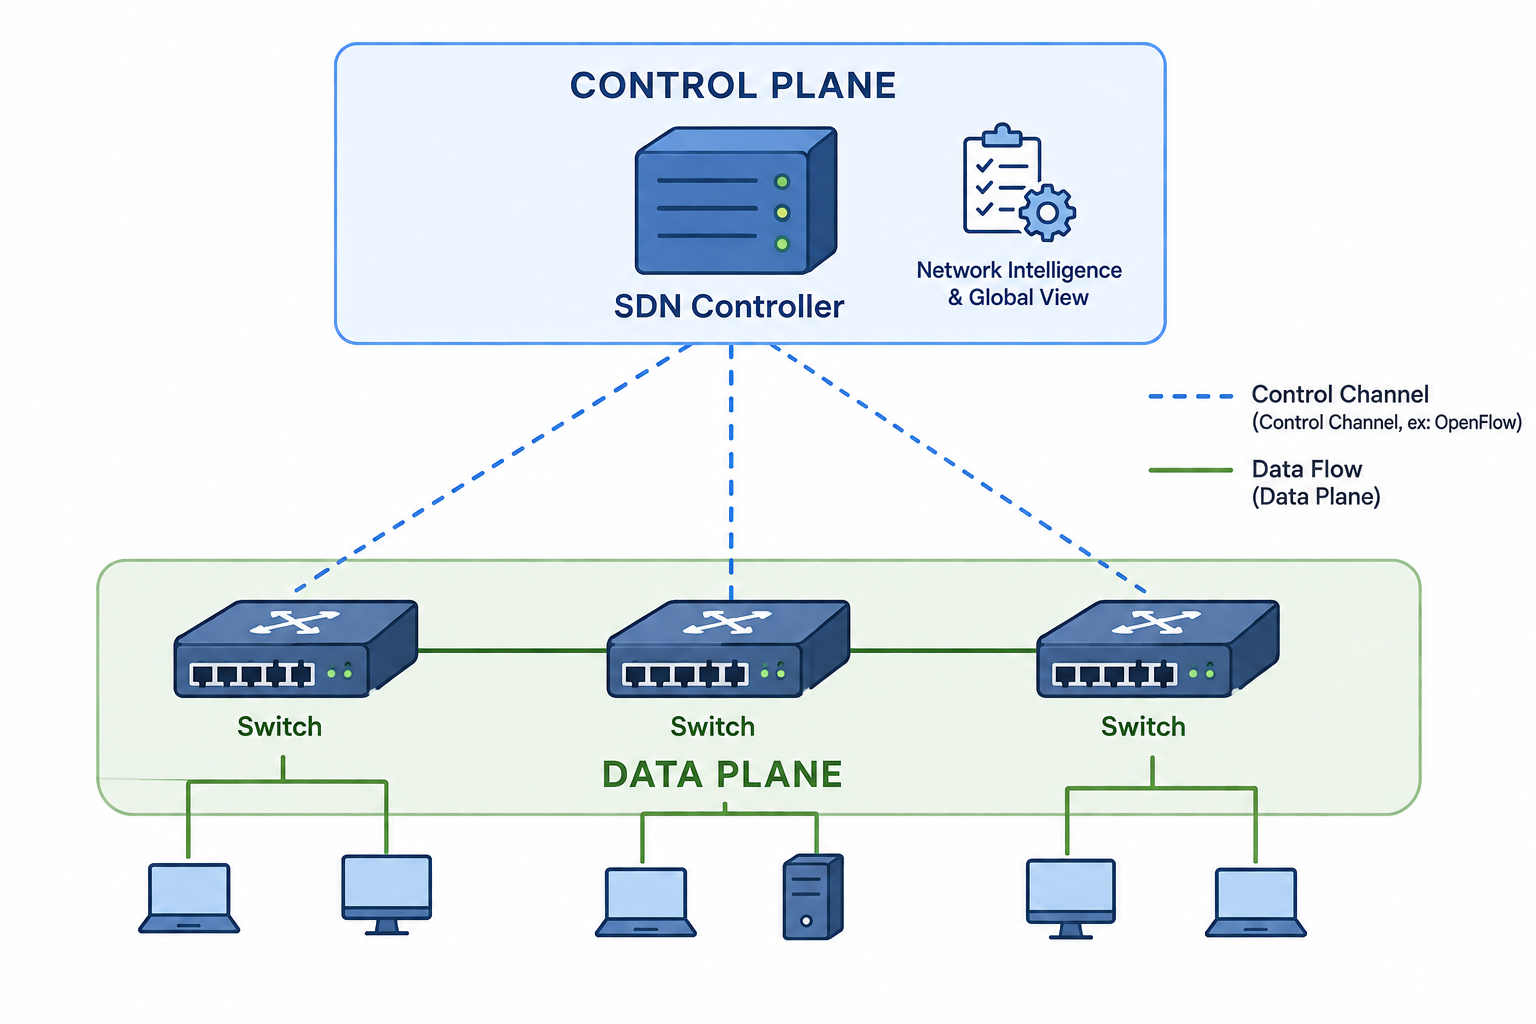
\includegraphics[width=0.8\textwidth]{images/sdn_architecture_v2.png}
    \caption{Software-Defined Networking architecture: the control plane is
    decoupled from the data plane and programs the forwarding devices through
    the OpenFlow protocol.}
    \label{fig:sdn_architecture}
\end{figure}

\subsection{Containerisation and Docker}
Containers package an application with its dependencies and share the
host kernel, which makes them lighter to provision and tear down than
virtual machines, a property that suits resource-constrained edge platforms.
On ARM-based edge devices, Kaiser et al. benchmark Docker, Podman, and
Singularity using computer-vision and data-science workloads typical of
edge scenarios, and find that Docker achieves near-native start-up times,
around 0.9 seconds, together with the best CPU and RAM utilisation for
most of the evaluated applications
\parencite{Kaiser2023BenchmarkingContainerTechnologiesARMEdge}.

    Orchestration of containerised applications has also been studied
across layers: Sofia et al. propose context-aware cross-layer
orchestration for containerised applications in decentralised edge-cloud
environments serving next-generation IoT services, treating contextual
information such as data freshness as part of the orchestration input
\parencite{Sofia2023DynamicContextAwareCrossLayer}.

    Orchestration tools must also adapt to the edge, and Cilic et al.
evaluate Kubernetes, the lightweight distributions K3s and KubeEdge,
and the ioFog platform in real edge execution environments, finding
that none of the evaluated tools monitors and schedules services based
on client QoS parameters, a logic that must be supplied externally,
and that challenges remain to fully adapt these cloud-designed tools
to dynamic edge environments
\parencite{Cilic2023PerformanceEvaluationContainerOrchestrationTools}.

    Taken together, these studies establish containers as a
provisioning unit well suited to constrained edge nodes, with start-up
cost as the quantity that matters when capacity must be added quickly.
Precisely because start-up itself is sub-second, the interval that
remains between readiness and first served traffic is not absorbed by
provisioning cost.

\subsection{NoSQL and MongoDB: The Storage Tier}\label{sec:platform_storage}
Document-oriented NoSQL stores organise data as schema-flexible
documents rather than as rows of relational tables. Because related
data is embedded in a single document and the model avoids joins and
fixed schemas, records can be partitioned and replicated across
servers, which is how these stores scale horizontally, whereas
relational systems are traditionally scaled vertically by enlarging a
single server. This model suits the heterogeneous data of edge and IoT
services, whose structure varies between sources and evolves over time.

    MongoDB is a document store of this family: it holds data as BSON
documents within collections and provides a flexible schema.
In MongoDB, redundancy is organised natively around the replica
set: a group of \texttt{mongod} processes that maintain the same
data set. One member is elected primary and serves the clients'
writes, which it records in an operation log; the remaining
members, the secondaries, replicate by applying that log
asynchronously. Members exchange heartbeats, and when the primary
fails or becomes unreachable, the secondaries hold an election and
promote one of their own, so the set keeps serving without
operator intervention. Members can also be added to and removed
from a deployment while it keeps serving, which turns the replica
set into a controllable unit of storage capacity rather than a
fixed configuration.

\begin{figure}[H]
    \centering
    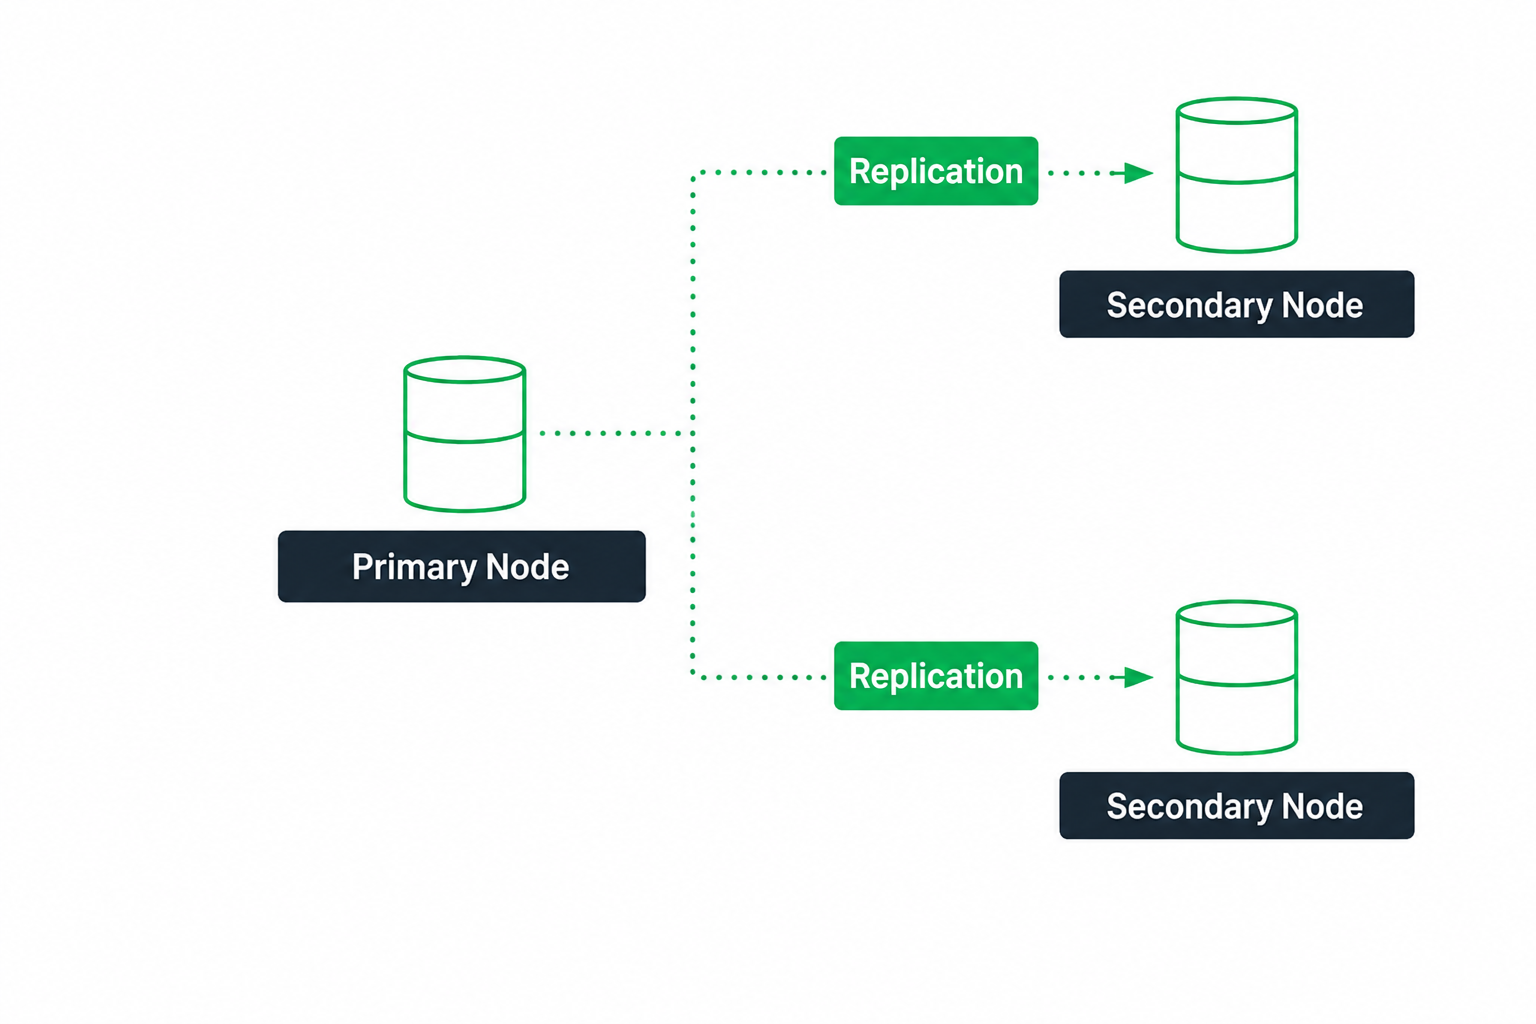
\includegraphics[width=0.7\textwidth]{images/mongodb_replica_set.png}
    \caption{MongoDB replica set: a primary member serving the clients and
    secondary members to which the data is replicated.}
    \label{fig:mongodb_replica_set}
\end{figure}

    Eyada et al. compare MongoDB against MySQL for IoT data management
and find that MongoDB outperforms the relational system in latency
across a wide range of IoT workloads
\parencite{Eyada2020PerformanceEvaluationIoTDataManagement}.

    Ferreira et al. survey databases in edge and fog environments,
dissecting the drivers for pushing storage towards the edge and the
mechanisms employed to deal with the challenges these environments
pose. In the study, surveyed systems rest on replication protocols
that maximise the latency advantage of geographical placement,
and the survey leaves the expansion of replica counts while
minimising the coordination overhead it incurs as an open
direction, adjacent to the storage capacity action this
dissertation evaluates
\parencite{MerujeFerreira2024DatabasesEdgeFogEnvironmentsSurvey}.

    Geo-distributed deployments combine replication with placement, and
Mealha et al. exemplify the frontier: their cloud/edge replication over the
MongoDB data model leaves a \enquote{dynamic placement strategy of
either full or partial databases} to future work
\parencite{Mealha2019DataReplicationCloudEdge}.

    Related work on the data side of the scaling loop, however, treats
placement and retention rather than a live scale-out decision.
Popularity-based placement distributes content according to access
frequency, but Wei and Wang describe their placement decision as static
and list online placement as future work
\parencite{Wei2023PopularityDataPlacementLoadBalancing}.

    Malazi et al. survey dynamic service placement in 
multi-access edge computing and record fragmented evaluation
practice across the field 
\parencite{TabatabaeeMalazi2022DynamicServicePlacementMultiAccess},
while placement re-optimises which node serves data rather than
selecting a capacity action. None of these works selects storage
scale-out from a live observed bottleneck, adding or removing
replica-set members while the deployment keeps serving, which is the
capacity action evaluated in the thesis.

\section{Monitoring \& Telemetry}\label{sec:lit_monitoring}
Monitoring and telemetry observe the state of a running service and
deliver that evidence to whoever acts on it. Monitoring is the
collection of resource and load metrics, telemetry the transport that
carries the collected data to the consumer, and together they form the
first link of the demand-to-capacity chain: every later decision, on
scaling or on routing, can act only on the evidence this link delivers,
at the time it delivers it, and with whatever intermediate observations
the delivery process preserves.
    In edge deployments the link matters doubly, because the
evidence must travel from many dispersed nodes to the decision point,
so any delay or gap in its delivery becomes delay or blindness in the
orchestration response. 

    The state of the art in this area is built around a common
pipeline: per-node collectors sample resource and load metrics, an
aggregation layer summarises the samples, and the resulting series feed
the consumers that make decisions. In orchestrators this pipeline is
standardised around periodic scraping into a time-series store, as in
OSM-based NFV for transparent VNF clusters, where the monitoring module
polls the infrastructure into a Prometheus database
\parencite{Llorens2021SDNBasedHorizontalAutoScalingLoadBalancing}.
Containerised edge stacks assemble the same building blocks in one place:
an SDN controller, a Kubernetes cluster, and a time-series database share
a single orchestration stack for industrial IoT, yet the monitoring
evidence reaches the time-series store through a dedicated power-meter
agent outside the cluster
\parencite{Okwuibe2020SDNEnhancedResourceOrchestrationContainerized}.

    Delivery is conventionally pull-based, the
consumer requesting the latest sample at a fixed interval
\parencite{Yaseen2025CountersTelemetrySurveyProgrammableNetwork}, and this
choice alone determines much of what the consumer can know: between two
collection instants the monitored state is unobserved, and what the
pipeline forwards between instants determines whether the consumer
receives the complete history, a complete but delayed history, or only
the latest state. These different forms are defined
as event-preserving delivery, delayed event-preserving delivery,
and latest-state delivery. Their effect on resource orchestration
is part of the subject of study in this thesis.

    The reviewed evidence spans three contexts in which this link has
been studied: cluster-federation monitoring, network telemetry, and
edge-platform observability. In each, the review asks whether the
delivery mechanism itself is varied, what downstream consequence the
variation is shown to produce, and what the work leaves as a given.

    Within cluster-federation monitoring, the collection interval has
been shown to be a genuine variable rather than a fixed parameter. AdapPF
\parencite{Huang2023AdapPFSelfAdaptiveScrapeInterval} varies the
Prometheus scrape interval of a geo-distributed Kubernetes federation and
measures the effect on a downstream consumer: under high load, a coarse
sixty-second interval substantially degrades scheduling accuracy relative
to a five-second interval, and an adaptive cadence restores it while
reducing cross-cluster monitoring traffic.
AdapPF is the only reviewed work that varies monitoring freshness and
measures a downstream consequence, but it stops at a single consumer, a
scheduler, and does not run over a stateful service. 

    The same line of work treats monitoring overhead as a
recognised bottleneck in geo-distributed deployments, proposing
aggregation so that monitoring can scale with the federation 
\parencite{Huang2024AggregateMonitoringGeoDistributedKubernetes},
aggregation being itself a form of summarisation that discards
intermediate observations. Within the same platform context, Zhou and
Yong study what to monitor rather than how it is delivered, comparing
custom-metric autoscaling driven by application-level failure rates
against conventional CPU-based autoscaling in Kubernetes, and find that
metric choice changes scaling quality under load, albeit on a small
single-service testbed \parencite{Zhou2024ImplementHPANginxServiceUsing}.

    A second context, network telemetry, converges on the same delivery
mechanics from the network side. Yaseen reviews programmable network-wide
monitoring and records that pull-based polling produces
\enquote{visibility gaps} between collection instants, calling for
monitoring to be \enquote{tightly integrated with network control and
automation} \parencite{Yaseen2025CountersTelemetrySurveyProgrammableNetwork}.
Industry practice points in the same direction: a production SDN
controller for 5G backhaul networks co-locates a telemetry collector with
a routing adjuster in a closed loop over the wide area
\parencite{Hung2022SDNControllerMonitoringArchitecture5G}, showing that
co-location of monitoring with control is feasible, although the loop
omits scaling altogether. 

    At the platform level, adjacent observability
work exhibits the same open dimension: Usman et al., surveying
observability of distributed edge and container-based microservices,
leave the definition of appropriate measurement intervals as an
open research topic
\parencite{Usman2022SurveyObservabilityDistributedEdgeAmp}.
None of these works runs over a stateful service, so they are read
here for the delivery mechanisms they expose, not as direct precedents
for the platform under study.

    Table~\ref{tab:monitoring_evidence} summarises the strength of the
evidence each of these works provides for the link under study.

\begin{table}[htbp]
    \centering
    \caption{Evidence for the link between monitoring and decision in the reviewed literature.}
    \label{tab:monitoring_evidence}
    \begin{tabular}{p{0.40\textwidth} p{0.16\textwidth} p{0.36\textwidth}}
        \toprule
        Work & Strength & What it shows \\
        \midrule
        Llorens-Carrodeguas et al. (2021) & Measured & Orchestration
        monitoring polls into Prometheus; delivery semantics not varied \\
        Okwuibe et al. (2020) & Measured & SDN controller, Kubernetes,
        and a time-series store share one stack; no delivery dimension \\
        AdapPF (Huang \& Pierre, 2023) & Measured & Freshness changes a
        scheduler's accuracy; no stateful-service or admission trace \\
        Huang \& Pierre (2024) & Measured & Aggregation contains
        monitoring overhead but discards intermediate observations \\
        Zhou \& Yong (2024) & Measured & Metric choice changes scaling
        quality; the delivery mechanism stays fixed \\
        Yaseen (2025) & Documented & Pull-based polling leaves visibility
        gaps; calls for monitoring integrated with control \\
        Hung et al. (2022) & Measured & Production controller co-locates
        telemetry and routing; scaling omitted \\
        Usman et al. (2022) & Surveyed & Appropriate measurement
        intervals remain an open research topic \\
        Belgaum et al. (2020) & Not addressed & A seventy-six-paper review of the
        adjacent load-balancing field lists no freshness issue among its
        open problems \\
        \bottomrule
    \end{tabular}
\end{table}

    Across the reviewed literature, therefore, the building blocks of the
delivery question appear separately: AdapPF varies the interval that
produces delay, Yaseen documents the gaps that polling leaves, and
aggregation summarises away intermediate observations, yet no reviewed
work distinguishes delayed event-preserving delivery from latest-state
delivery, and none traces either regime through a stateful service's
scaling and traffic-admission path.

\section{Auto Scaling}\label{sec:lit_auto_scaling}
Auto-scaling adjusts the amount of allocated resources to the load that
a service receives: when demand grows, additional capacity is
provisioned, and when demand recedes, surplus capacity is released, so
that the service keeps serving requests without holding resources it
does not use. In edge deployments the question gains more relevance 
because each site holds limited capacity and receives demand that
fluctuates over time, so when and how many resources
to add or remove determines both the quality of service during
a demand shift and the efficiency with
which scarce resources are managed.

% \begin{figure}[H]
%     \centering
%     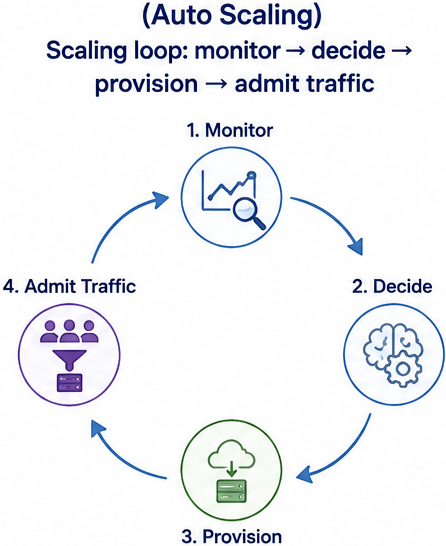
\includegraphics[width=0.55\textwidth]{images/autoscaling_loop.png}
%     \caption{Closed loop of an autoscaler: monitoring, analysis, planning,
%     and execution repeated over the managed service.}
%     \label{fig:autoscaling_loop}
% \end{figure}

    The field show what the surveyed
auto-scalers have in common. Qu et al. classify them along the scaling
indicator, the resource estimation method, and the timing of the action,
and Taherizadeh and Stankovski organise the same questions across edge
application types and operational challenges. In both, the unit surveyed
is the scaling of service instances, whether virtual machines or
containers: the questions the field asks are when to scale and how many
instances to add, and which kind of capacity is provisioned is not among
the classification dimensions
\parencite{Qu2018AutoScalingWebApplicationsClouds,Taherizadeh2017AutoScalingApplicationsEdgeComputing}.

    When SDN enters the loop, the traffic side is added, but the scaled
resource remains the one the service function is built from:
Llorens-Carrodeguas et al. couple SDN-based traffic steering with
horizontal scaling of a transparent VNF cluster, so that a single
controller re-programs the forwarding paths while instances of the same
pre-dimensioned function pool are activated or deactivated according to
their load and CPU status
\parencite{Llorens2021SDNBasedHorizontalAutoScalingLoadBalancing}.
The decision reduces to whether and how many instances of that one
function to activate, and the service model contains no data tier on
which those instances depend. A stateful edge service differs precisely
on that point: its replicas depend on a data tier that is itself live
capacity, and when the limiting resource is that data tier, adding
instances does not relieve the pressure that sits there.

    Predictive and learning-based approaches sharpen the same decision
without widening it: Toka et al. formalise the Kubernetes horizontal
autoscaler's control model to anticipate demand for edge clusters
\parencite{Toka2021MachineLearningScalingManagementKubernetes}, Ju et
al. and Cheng et al. forecast workload to adjust replica counts ahead of
demand, the latter jointly with placement
\parencite{Ju2021ProactiveAutoscalingEdgeComputingSystems,Cheng2023ProScaleProactiveAutoscalingMicroserviceTime},
and Li et al. couple scaling and placement in a single optimisation
\parencite{Li2021JointOptimizationAutoScalingAdaptive}. Across these
systems the unit whose count is forecast and adjusted is the compute
replica. The improvement they pursue is a better forecast of how many
instances to run; which tier holds the limiting resource does not enter
their problem.

    Scaling one resource does not always make the service better,
because the pressure may sit elsewhere. Nikravesh et al. quantify what
that default costs in a three-tier web service: the scaling decisions
taken for the business tier turn out to be insensitive to database
capacity, yet reducing database capacity raises the rate of SLA
violations, so service quality can be governed by the tier that the
scaling decisions ignore
\parencite{Nikravesh2017ImpactDatabaseLayerAutoScaling}. Dogani et
al. record the same boundary across the systems they survey: adding
resources does not necessarily raise throughput when the bottleneck
lies elsewhere
\parencite{Dogani2023AutoScalingTechniquesContainerCloud}. Among those
systems, awareness of the effect is scarce and cross-service only:
Waterfall, a machine-learning auto-scaler, accounts for how scaling
one microservice can shift the bottleneck towards downstream services,
and ATOM uses layered queuing networks to reduce bottleneck shifts in
model-agnostic controllers
\parencite{Dogani2023AutoScalingTechniquesContainerCloud}. Both
provisions remain compute-side: the data tier, even when it is the one
driving the violations, is not part of the action space the reviewed
systems expose.

    The most recent systems sharpen the same boundary: PBScaler identifies
the microservice whose degradation propagates through the call graph,
ranks candidate bottlenecks, and optimises replica management around the
identified bottleneck
\parencite{Xie2024PBScalerBottleneckAwareAutoscalingFramework}.
Bottleneck awareness therefore exists in the current state of the art,
but the bottleneck it locates is always a microservice and the action it
takes is always a compute-replica count. When the limiting resource is
the data store rather than any microservice, locating the bottleneck is
not enough: the action must change kind.

    The closest reviewed precedent to selecting between resource tiers
is the provisioning model of Li et al., which adds both cloud compute
instances and data replicas in cloud-assisted edge systems, from a
forecast of future workload built over historical workload data
\parencite{Li2020HeterogeneityAwareElasticProvisioningCloud}. Both
actions are available, but the trigger is a forecast rather than a live
observed bottleneck, and the outcome is measured in tenancy cost and
utilisation rather than in user service quality and resource
management efficiency. 

    Pelle et al. keep function and state placement in sync through
an integrated optimisation over an edge platform
\parencite{Pelle2022CostLatencyEdgePlatform}. The mechanism is
placement rather than live capacity action: state is moved to follow
the functions, while the response to an observed bottleneck remains
outside the optimisation.

    The most recent survey converges on the same boundary: El Mrabet et
al. extend the classification across cloud, fog, and edge, categorising
the surveyed methods by their decision mechanism, scaling strategy, and
deployment layer, and the provisioned tier is not among the
classification dimensions
\parencite{ElMrabet2025ComprehensiveSurveyTaxonomyAutoscalingTechniques}.
The field's own framing expresses the same default:
Qu et al. describe the web application as split into
application logic and a database tier, and
record that \enquote{the database tier is often considered dynamically
unscalable and ignored by auto-scalers}
\parencite{Qu2018AutoScalingWebApplicationsClouds}.

\begin{table}[htbp]
    \centering
    \caption{Evidence on capacity-action selection in the reviewed literature.}
    \label{tab:autoscaling_evidence}
    \begin{tabular}{p{0.40\textwidth} p{0.16\textwidth} p{0.36\textwidth}}
        \toprule
        Work & Strength & What it shows \\
        \midrule
        Qu et al. (2018) & Surveyed & Canonical taxonomy of when and how many
        to scale; database tier ignored by the surveyed auto-scalers \\
        Taherizadeh \& Stankovski (2017) & Surveyed & Edge-specific
        taxonomy; scaling surveyed over service instances \\
        Llorens-Carrodeguas et al. (2021) & Measured & SDN steering coupled to
        horizontal VNF scaling; capacity-action type fixed \\
        Toka et al. (2021) & Measured & Learning improves Kubernetes edge
        scaling; compute-only with the metrics pipeline taken as given \\
        Cheng et al. (2023) & Measured & Instance counts and placement
        jointly optimised; provisioned unit remains compute \\
        Nikravesh et al. (2017) & Measured & Database capacity ignored by
        the business-tier autoscaler, yet it drives the SLA violations \\
        Dogani et al. (2023) & Surveyed & Bottleneck-shift awareness exists,
        compute-only and cross-service; no storage action \\
        PBScaler (2024) & Measured & Bottleneck-aware replica
        management; the bottleneck is a microservice, the action remains
        compute \\
        Li et al. (2020) & Measured & Compute instances and data replicas
        provisioned together, but from a forecast, not a live bottleneck \\
        El Mrabet et al. (2025) & Surveyed & Recent taxonomy; the
        provisioned tier is not among the classification dimensions \\
        \bottomrule
    \end{tabular}
\end{table}

    Taken together, this evidence establishes first that the kind of
capacity added can matter. Adding compute replicas cannot relieve pressure
whose limiting resource lies in the data tier; database capacity can govern
SLA violations while a compute-tier scaling decision remains unchanged; and
bottleneck-aware compute systems already improve their decisions by locating
which microservice constrains the request path. Capacity actions are therefore
not interchangeable merely because each adds resources.

    The unresolved step appears when monitoring can identify more than one
class of bottleneck and the platform exposes a corresponding remedy for each.
The reviewed taxonomies still organise auto-scaling around when to scale and
how many resources to add, while the provisioned tier remains an architectural
given. Where compute and data resources enter the same problem, they are
jointly provisioned from forecasts or jointly placed, rather than selected at
runtime as alternative actions conditioned on a live compute-bound or
data-access-bound bottleneck. What is left uncharacterised is therefore not
whether the action matched to the observed bottleneck helps, but how much:
how the benefit is distributed across targeted-tier relief, service recovery,
and resource use; where mismatched fixed policies pay the cost of their
choice; and how reliably a telemetry-driven selector commits to the right
single action. 
    
    Equally unexamined is the boundary at which
the decision is fed: where the reviewed
works describe the monitoring and lifecycle components that supply the
scaling decision at all, they leave those components outside the decision
loop, a default examined across all three interfaces in
\ref{sec:lit_three_layer_separation}.

    Works that do couple compute with data do so at design time
or from forecasts, in the strand reviewed in
\ref{sec:platform_storage}.

% Aqui
\section{Load Balancing on SDN}\label{sec:lit_sdn_lb}
Load balancing distributes incoming traffic among a set of available
backends so that no single backend is overloaded while others remain
idle. In SDN networks this distribution is programmed centrally: the
controller installs forwarding rules that steer each flow to a
selected backend, and a selection policy decides which backend
receives the next flow. The function matters at the edge because a
newly provisioned backend only becomes usable capacity once traffic
actually reaches it, so how backends enter and leave the pool of
candidates is part of the problem itself.

\begin{figure}[H]
    \centering
    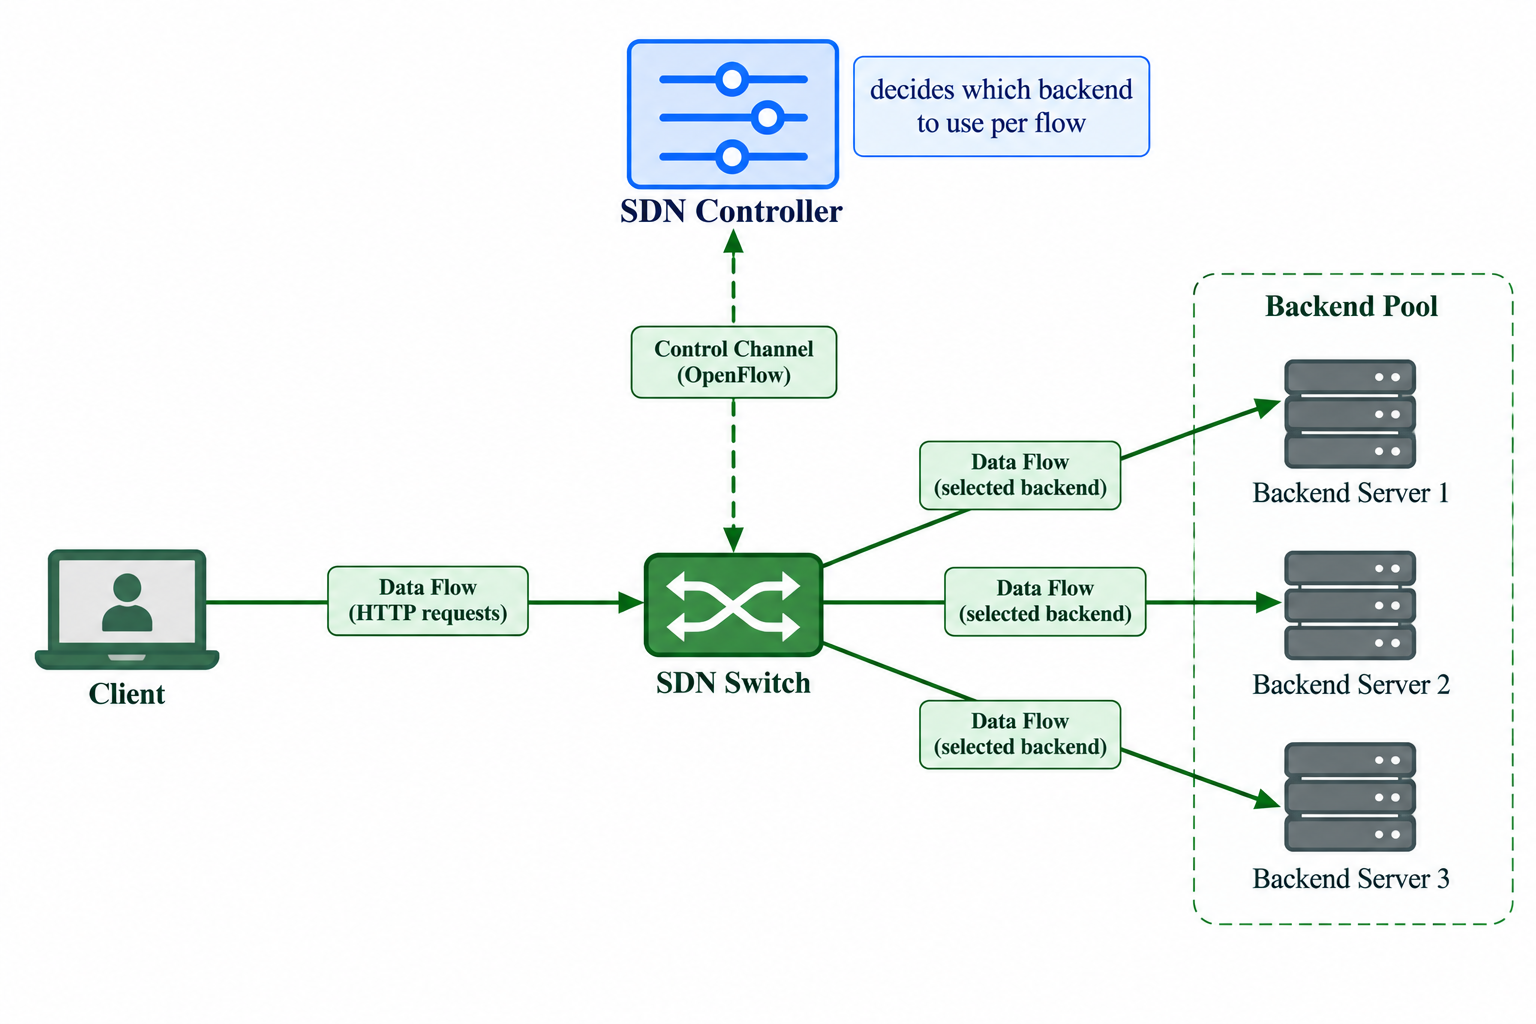
\includegraphics[width=0.7\textwidth]{images/sdn_load_balancing_v2.png}
    \caption{Load balancing in an SDN network: the controller installs
    forwarding rules that distribute client traffic among the available
    backends.}
    \label{fig:sdn_load_balancing}
\end{figure}

\subsection{Selection and Backend Membership}
    At a given routing decision, a load-balancing policy must operate over
the set of backends currently eligible to receive traffic. Treating this
set as fixed for that decision is therefore a valid modelling boundary
rather than a limitation of the selection policy. The SDN load-balancing
literature accordingly concentrates on how to select a backend from the
available candidates, using criteria such as load, path properties, and
resource utilisation
\parencite{Neghabi2018LoadBalancingMechanismsSoftwareDefined,Belgaum2020SystematicReviewLoadBalancingTechniques}.

    The set of eligible backends may nevertheless change between routing
decisions. This change does not alter the selection problem itself; it
creates a separate lifecycle responsibility. A backend must be provisioned,
become able to serve the application, have that state propagated to the
routing plane, and be included in the eligible set before the next routing
decision can select it. The interval between verified readiness and routing
eligibility is therefore an admission delay, not a property of the
backend-selection algorithm.

\subsection{Admission as a Lifecycle and Discovery Interface}
    Service-discovery research distinguishes publication or registration,
discovery, resolution to an endpoint, and maintenance of service
information. It also recognises that dynamic services may join or leave
and that the freshness of maintained information can affect availability
and delay
\parencite{Pourghebleh2020ServiceDiscoveryInternetThingsReview,Achir2022ServiceDiscoverySelectionIoTSurvey}.
These concerns are adjacent to the present problem, but they do not by
themselves measure when a newly ready compute backend becomes eligible for
traffic in an elastic SDN service.

    Production systems mechanise the same interface, generally as one step
within a broader lifecycle rather than as an independently varied factor.
Shard Manager, the framework that manages Facebook's geo-distributed
sharded applications, treats readiness as an explicit, ordered step of
the shard lifecycle: it negotiates with the cluster managers about when
to safely execute container lifecycle operations and ensures that an
application drops no request during a graceful shard migration, with
the readiness-to-traffic transition performed through a service-discovery
map. Its unit, however, is shard-role migration rather than
container-readiness admission, and the propagation semantics of the
transition are part of that unit rather than an independently varied
factor in its evaluation
\parencite{Lee2021ShardManager}. On the routing side, Kurma, a load
balancer for geo-distributed storage systems, is explicitly designed to
operate at a granularity of seconds so that it can \enquote{work in
tandem with modern elastic controllers, thereby reducing over-provisioning
and SLO violations incurred during provisioning delays}
\parencite{Bogdanov2018Kurma}. The delay between provisioning and usable
capacity is therefore a recognised cost in production routing, yet the
unit of analysis in both systems is the broader lifecycle: the interval
in which readiness state propagates to the routing plane is not
separated from it.

    The closest architectural antecedent is Llorens-Carrodeguas et al.,
whose SDN redirector combines monitoring, auto-scaling, and load balancing
for a transparent VNF cluster. Their system changes the number of active
cluster members and removes flow rules for unhealthy instances using
status obtained through the MANO monitoring path
\parencite{Llorens2021SDNBasedHorizontalAutoScalingLoadBalancing}.
It therefore demonstrates that dynamic membership is already a legitimate
concern. Its evaluation, however, reports activation at the granularity of
the integrated system, so the interval from verified application readiness
to routing eligibility is not separated from the surrounding lifecycle.

    Across this literature, therefore, the selection of a backend among
eligible candidates is well characterised, and integrated systems implement
broader membership transitions. What remains unisolated in the reviewed
literature is the post-readiness handoff from lifecycle completion to actual
traffic contribution under controlled invariants. This is the gap RQ3
isolates: the dissertation varies readiness-admission coordination while
holding the application-readiness criterion and selection function constant,
and measures the time until newly provisioned capacity becomes selectable
and serves traffic. Direct lifecycle notification and periodic discovery are
the two operational realisations of that coordination interface.

\section{SDN-Based Orchestration Platforms}\label{sec:lit_sdn_orchestration}
Resource orchestration is the management layer that keeps a running
service within its requirements by coordinating the compute, network,
and storage resources of the infrastructure on which it runs. It is
the activity that the technologies and tools reviewed in
\ref{sec:platform_background} are assembled to serve: edge sites
supply the resources, SDN supplies the programmable connectivity,
containers supply the unit of compute, and the document store holds
the service state. That decision-making, and its execution, is
orchestration, and at the edge it is the more demanding because each
site holds scarce capacity and the demand on it fluctuates over time.
Because the service is stateful, the capacity action is itself
two-sided: compute replicas serve requests, while the data they serve
lives in the storage tier, so scaling can address either side.

    This dissertation studies the SDN-based form of this management
layer, in which the coordination spans the SDN controller, the
container runtime, and the data store, and the challenge is to keep
these layers working together as demand moves across sites. The
platforms reviewed here bind these layers with different degrees of
coupling, and this section examines how closely the three functions
of the demand-to-capacity chain, monitoring, scaling, and routing,
are held together in each, using the terms interface and coordination
gap as defined in \ref{sec:context_motivation}.

    Along the layers axis, edge orchestration is cross-layer by
construction. Baktir et al. organise the gains that SDN brings to
edge computing into benefit areas such as centralised visibility and
programmatic traffic management
\parencite{Baktir2017HowCanEdgeComputingBenefit}; Wang et al. survey
architectures in which SDN and NFV jointly coordinate placement,
traffic, and caching across the network and service layers, showing
that SDN's role at the edge extends beyond forwarding into
orchestration
\parencite{Wang2019SoftwareDefinedNetworkingEnhancedEdge}; and Sofia
et al. build context-aware cross-layer orchestration for
containerised edge-cloud applications
\parencite{Sofia2023DynamicContextAwareCrossLayer}.

    The surveyed stacks bind these layers into concrete deployments.
Okwuibe et al. assemble the stack closest to the one built in this
dissertation: an SDN controller, a Kubernetes cluster, and a
time-series database serve containerised industrial-IoT edge
applications, while a MongoDB instance stores the sensor data. The
three functions nevertheless remain separate components, and the
study does not causally connect that separation to any
service-quality implications
\parencite{Okwuibe2020SDNEnhancedResourceOrchestrationContainerized}.
Peng et al. exercise SDN-based resource management in vehicular
multi-access edge computing as task migration and radio slicing,
treating telemetry as available input rather than as an interface to
be studied, and without container orchestration or tier scaling
\parencite{Peng2019SDNResourceManagementAutonomousVehicular}.

    A recurring minority of these platforms co-locates the functions
at the SDN control point itself. Llorens-Carrodeguas et al. combine
monitoring, auto-scaling, and load balancing in a single SDN
redirector for a transparent VNF cluster, although metric collection
and the lifecycle operations that feed and execute the decision
remain external
\parencite{Llorens2021SDNBasedHorizontalAutoScalingLoadBalancing};
a production SDN controller for 5G backhaul co-locates a telemetry
collector with routing adjustment in a closed loop, omitting scaling
altogether
\parencite{Hung2022SDNControllerMonitoringArchitecture5G}. The first
arrangement binds all three functions at one control point, the
second binds two of the three, and the Okwuibe stack shows the full
assembly in one deployment while keeping the functions as separate
components. Co-location at the SDN control point is therefore a
feasible, precedented arrangement rather than an invention of this
dissertation.

% \begin{figure}[H]
%     \centering
%     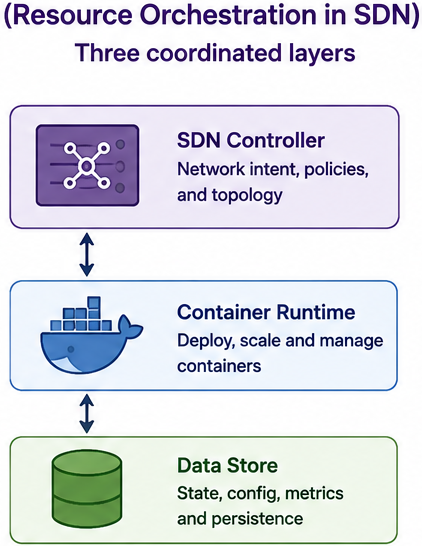
\includegraphics[width=0.7\textwidth]{images/orchestration_layers.png}
%     \caption{Layered orchestration of containerised services over an
%     SDN-programmed edge infrastructure.}
%     \label{fig:orchestration_layers}
% \end{figure}

    At the geo-distributed scale, three systems coordinate the same
functions by construction, and they delimit the claim of this
dissertation. OneEdge replaces a centralised control plane with a
hybrid one that propagates aggregate state across sites, keeping its
control loops coordinated through shared state
\parencite{Saurez2021OneEdge}. McK8s shares Kubernetes
custom-resource state across four controllers of a geo-distributed
federation, so the loops never operate without shared state
\parencite{Tamiru2021Mck8sOrchestrationPlatformGeoDistributed}.
Kurma couples routing with elasticity by design: its load-balancing
decisions run at second granularity precisely to hold SLO violations
down while elastic controllers provision capacity
\parencite{Bogdanov2018Kurma}. These systems show that coordinated
control planes exist; none of them varies the delivery of demand
evidence, the selection of a capacity action, or the mechanism by
which ready capacity enters the routing pool as an independent
variable.

    The related background is therefore organised in two modes. In the dominant
mode, monitoring, scaling, and routing are implemented as separate
components, each running its own control loop, so the evidence and
commands that tie them together must cross component boundaries. The
separation is visible even in the tools themselves: the orchestration
platforms evaluated by Cilic et al. cannot re-schedule from dynamic
QoS parameters, so the tracking of QoS and the customisation of
scheduling logic must be performed by an external component
\parencite{Cilic2023PerformanceEvaluationContainerOrchestrationTools}.
In a second, recurring mode, the same functions are co-located at an
SDN-based control point or coordinated through shared state. What
neither mode provides, however, is a controlled decomposition in which
one handoff is varied while the others are held fixed. Prior systems
measure complete control processes or coordinate them by construction;
they do not isolate the contribution of telemetry delivery, capacity-action
selection, or readiness admission to the demand-to-capacity path. This
interface-level contribution is precisely the quantity this dissertation
highlights.

    SDN-based resource orchestration is therefore an established and
feasible arrangement, and the coordination it rests on is a recorded
open issue: Nain et al. list the coordinated management of resources
across the SDN-based edge among the continuing challenges of the
field
\parencite{Nain2024ResourceOptimizationEdgeSDNEdge}. The handoff
delay studied in this dissertation is one measurable dimension of
that coordination, and because the functions meet at boundaries that
an SDN-based control point can expose as explicit, configurable
interfaces, such a platform is a suitable experimental basis for
evaluating the handoff delays between them. The arrangement built in
this dissertation does exactly that: two peer SDN controllers host
controller-side telemetry consumption, scaling decision-making, and
routing within their respective control processes. Aggregated
telemetry arrives through an explicit, configurable delivery
interface, while policy and lifecycle hooks expose capacity-action
selection and readiness admission as independently variable
dimensions. The corresponding timing segments can therefore be
measured in isolation, as presented in \ref{ch:system_architecture}.

\section{The Unexamined Default: Independent Control Loops}\label{sec:lit_three_layer_separation}
Across the areas reviewed so far, the dominant mode
identified in \ref{sec:lit_sdn_orchestration} stands out: monitoring,
scaling, and routing are implemented as separate components, each
operating under its own control loop, so the information that ties
them together must cross component boundaries. This section examines
that default and what the reviewed work does and does not say about
it.

% \begin{figure}[H]
%     \centering
%     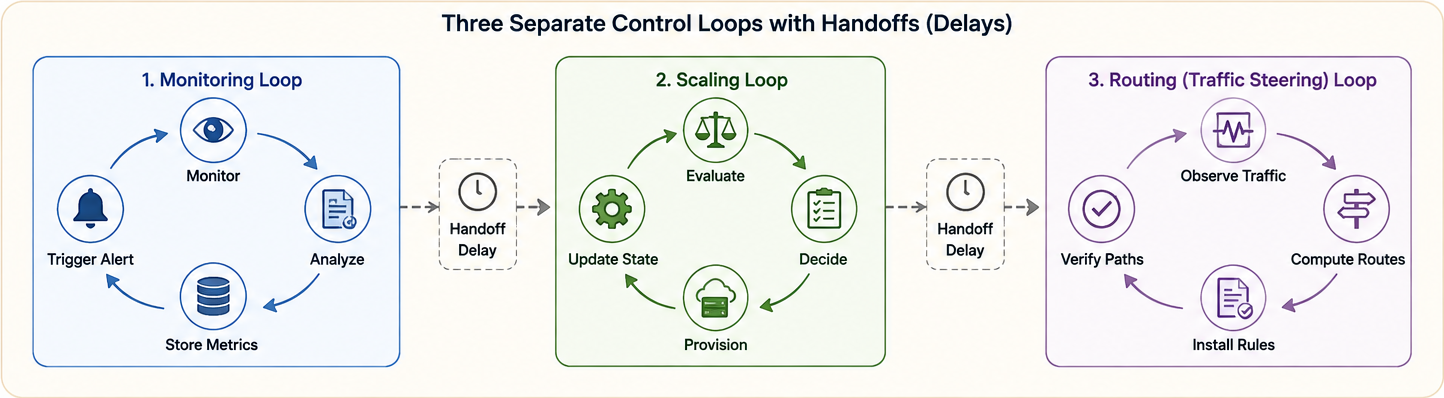
\includegraphics[width=0.9\textwidth]{images/independent_control_loops.png}
%     \caption{Independent control loops for monitoring, scaling, and routing:
%     the information that links them must cross component boundaries at each
%     handoff.}
%     \label{fig:independent_control_loops}
% \end{figure}

    The default recurs across the platform families this chapter has
used as context. In Kubernetes-based stacks, the reviewed work keeps
monitoring, scaling, and service routing as separate components:
Zhou and Yong drive the Kubernetes autoscaler with custom metrics,
Toka et al. model that autoscaler in isolation, and Okwuibe et al.
assemble an SDN controller, a Kubernetes cluster, and a time-series
store as one stack whose pieces exchange evidence rather than state
\parencite{Zhou2024ImplementHPANginxServiceUsing,Toka2021MachineLearningScalingManagementKubernetes,Okwuibe2020SDNEnhancedResourceOrchestrationContainerized}.

    In NFV MANO, metric collection and the lifecycle operations that feed
and execute the scaling decision remain external to it, and the
SDN-based redirector that closes the loop reads their outputs instead
of sharing their state
\parencite{Llorens2021SDNBasedHorizontalAutoScalingLoadBalancing}.

    In multi-access edge computing, dynamic service placement is surveyed
as a standalone problem, evaluated through user-facing metrics such as
latency, resource utilisation, and throughput, with no measure of the
time between the management functions themselves
\parencite{TabatabaeeMalazi2022DynamicServicePlacementMultiAccess}.
The separation is therefore not an artefact of one platform family
but the shared default; what varies across the surveyed areas is only
how far each acknowledges the boundaries it imposes.

    What none of the reviewed work does is isolate those boundaries.
Yaseen's call for monitoring to be \enquote{tightly integrated with
network control and automation} names the symptom
\parencite{Yaseen2025CountersTelemetrySurveyProgrammableNetwork};
Llorens-Carrodeguas et al. and Hung et al. bring two of the three
functions together without varying what crosses the remaining
boundary
\parencite{Llorens2021SDNBasedHorizontalAutoScalingLoadBalancing,Hung2022SDNControllerMonitoringArchitecture5G};
and the platforms that do coordinate across these functions, OneEdge,
McK8s, and Kurma, coordinate by construction rather than by studying
the interfaces
\parencite{Saurez2021OneEdge,Tamiru2021Mck8sOrchestrationPlatformGeoDistributed,Bogdanov2018Kurma}.

    Within the reviewed literature, therefore, the separation is documented
but not measured: no study varies one interface of the
demand-to-capacity chain while holding the others fixed. This
dissertation does not argue that the coordination gap is universal,
only that, within the reviewed literature, the interfaces that
compose it have not been isolated as independent variables; making
them isolable and measurable is the program of
Chapter~\ref{ch:system_architecture}.

\section{Synthesis and Research Gaps}\label{sec:lit_synthesis}
    The review travelled through the functions of resource
orchestration and asked, of each area, how the interfaces of the
demand-to-capacity chain are treated. The answer is consistent.
Monitoring and telemetry studies the collection and delivery of demand
evidence, yet the delivery mechanism itself remains a given: no reviewed
work distinguishes delayed event-preserving delivery from latest-state
delivery and traces both through a stateful service's scaling and admission
path. Auto-scaling evidence establishes that capacity kind matters: scaling
one tier can fail to relieve pressure in another, and database capacity can
govern service degradation even when the compute-tier decision is unchanged.
Yet when several resource actions are available, reviewed systems jointly
optimise a forecast resource mix or placement rather than select at runtime
between bottleneck-specific compute and storage remedies
\parencite{Qu2018AutoScalingWebApplicationsClouds,Nikravesh2017ImpactDatabaseLayerAutoScaling,Li2020HeterogeneityAwareElasticProvisioningCloud}.
Load-balancing systems implement integrated membership
transitions, but the reviewed work does not isolate the post-readiness handoff
to traffic contribution under controlled invariants. Finally, orchestration
platforms either leave these functions separated or coordinate them by
construction; neither mode varies one interface while holding the others
fixed.

    Table~\ref{tab:interface_gaps} condenses these findings into the
three interfaces and the question each leaves open.

\begin{table}[htbp]
    \centering
    \caption{The three interfaces of the demand-to-capacity chain and
    the questions they leave open.}
    \label{tab:interface_gaps}
    \begin{tabular}{p{0.34\textwidth} p{0.58\textwidth}}
        \toprule
        Interface & Open question \\
        \midrule
        Telemetry delivery to decision (RQ1) &
        Does a controller behave differently when demand evidence
        arrives late but complete, versus when intermediate
        observations are absent? \\
        Decision to capacity action (RQ2) &
        When compute and storage actions are both available, how much does
        selecting the action matched to an observed compute-bound or
        data-access-bound bottleneck change targeted-tier relief, service
        recovery, and resource efficiency relative to fixed single-tier
        policies, and where do the effects concentrate? \\
        Ready backend to traffic (RQ3) &
        How does readiness-admission coordination affect the delay from
        verified readiness to usable capacity and its transition-window
        service consequence? \\
        \bottomrule
    \end{tabular}
\end{table}

    Across the reviewed studies, the three interfaces are documented
in passing, their symptoms observed, and their study called for. The
cross-field connection is clearest where monitoring speaks of visibility
gaps between collection instants and service discovery speaks of registry
freshness. These are related formulations of stale control state, but the
reviewed work does not isolate how either interface contributes to the
end-to-end realization of usable capacity
\parencite{Yaseen2025CountersTelemetrySurveyProgrammableNetwork,Pourghebleh2020ServiceDiscoveryInternetThingsReview}.
The research questions of \ref{sec:research_questions} are the
experimental form of Table~\ref{tab:interface_gaps}.

    The evaluation follows the same per-interface discipline. Each
research question varies one interface while holding the other two
constant, and the findings are reported interface by interface rather
than summed into a single coordination penalty: the
demand-to-capacity chain is treated as a sequence of separately
measured interfaces, whose aggregate cost this dissertation
deliberately does not claim. The questions also sit between the
surveyed fields rather than inside any of them: each area's
abstraction serves its own question, and no surveyed platform
exposes the interfaces as independently tunable dimensions.
Chapter~\ref{ch:system_architecture} presents the platform designed
to make them askable and measurable.


\chapter{Architecture and Design of the Proposed Solution for Edge Services}\label{ch:system_architecture}
This chapter presents the architecture and design of the proposed
cross-layer \ac{SDN} orchestration platform for stateful edge services.
The design provides an experimental environment in which traffic steering,
controller-side telemetry consumption, and elasticity coordination operate
within each domain's controller process. The delivery of aggregated telemetry
and the lifecycle transitions from capacity action to traffic admission remain
explicit observation points. It is not intended to establish the general
superiority of a particular orchestration platform; the evaluation of the
mechanisms described in this chapter is presented in Chapter~5.

    Section~\ref{sec:design_requirements} defines the requirements that guided
the proposed solution. Section~\ref{sec:architecture_overview} presents the
two-domain architecture and its communication paths.

\section{Design Requirements}\label{sec:design_requirements}
The platform was designed to support stateful edge services whose demand and
resource requirements vary over time. Its design is guided by the following
requirements.

\begin{enumerate}[label=\textbf{DR\arabic*:}, leftmargin=*]
    \item \textbf{Cross-layer coordination.} Within each domain, traffic
    steering, telemetry consumption, topology awareness, and resource lifecycle
    management must exchange controller state through the same process.
    Aggregated telemetry must reach the controller through a structured,
    configurable delivery interface. Peer controllers must share the topology
    state needed for cross-domain awareness.

    \item \textbf{Separability of control interfaces.} The delivery of demand
    evidence, the selection of a capacity action, and the admission of ready
    capacity to traffic must remain independently configurable.

    \item \textbf{Independent compute and storage elasticity.} The platform
    must distinguish an increase or decrease in edge-service capacity from an
    increase or decrease in storage capacity, allowing each resource tier to
    be managed separately.

    \item \textbf{Lifecycle-safe admission.} Provisioned resources must not be
    regarded as usable capacity until the relevant readiness condition has been
    reached and the resource has been admitted to the appropriate routing path.

    \item \textbf{Fast-path isolation.} Packet handling must remain separate
    from slow infrastructure operations, such as container creation, replica
    preparation, and resource removal.

    \item \textbf{End-to-end observability.} The platform must record the path
    from demand observation to the first successful request served by newly
    available capacity.
\end{enumerate}

\section{Architecture}\label{sec:architecture_overview}

\begin{figure}[H]
    \centering
    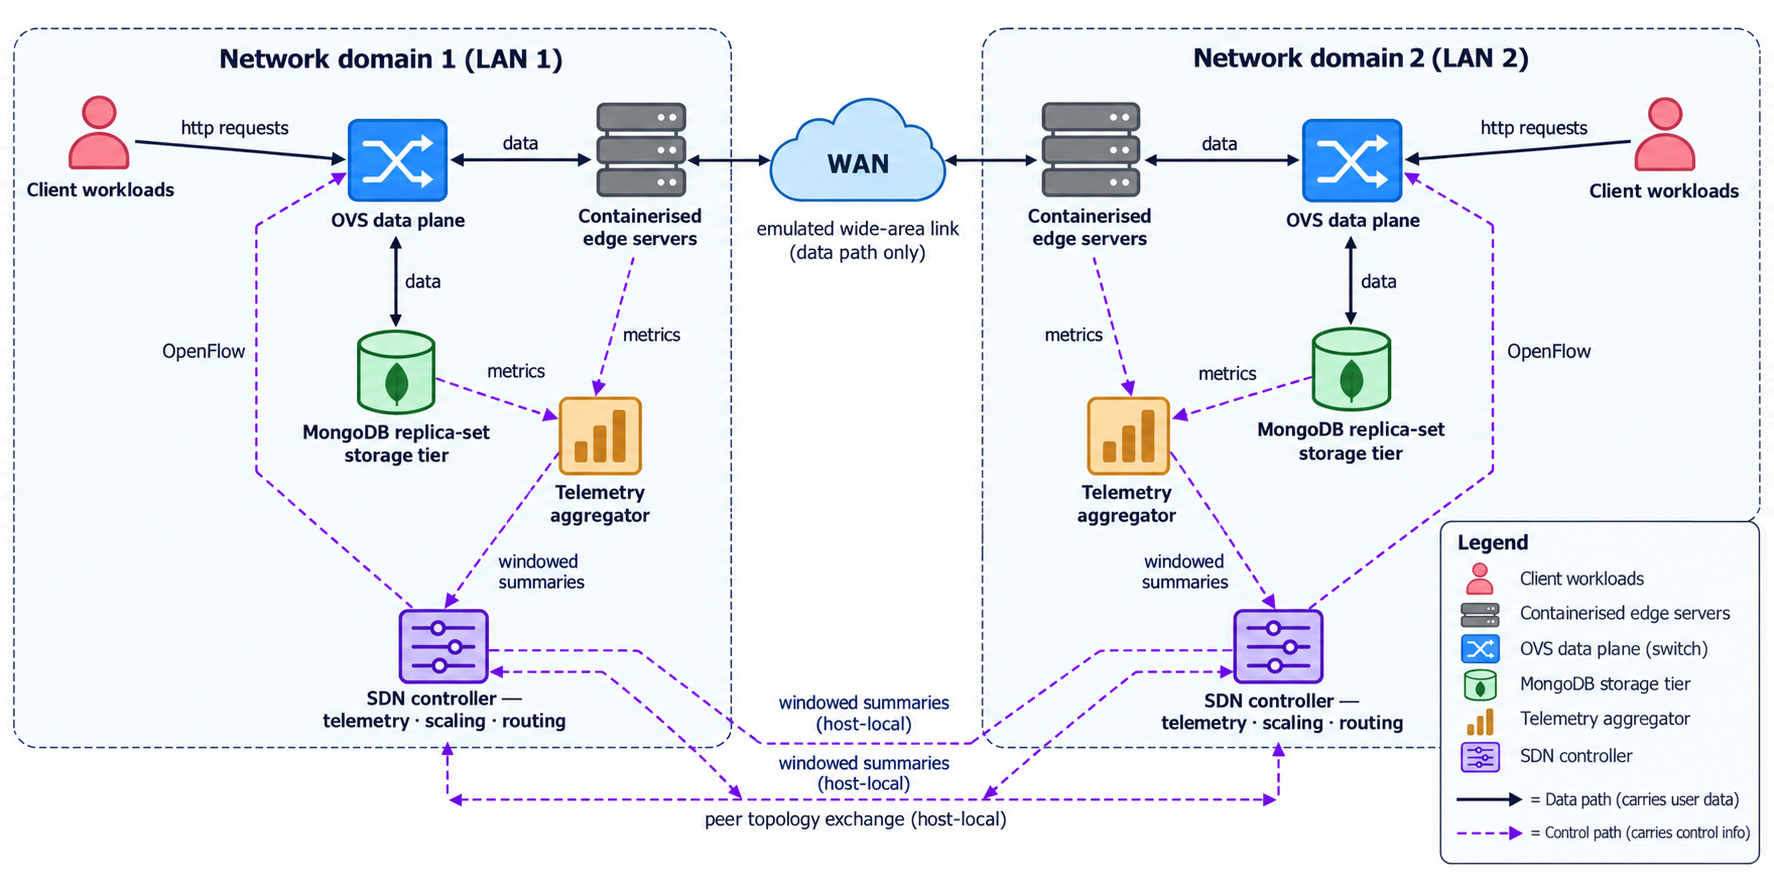
\includegraphics[width=0.95\textwidth]{images/architecture_overview.png}
    \caption{Architecture of the proposed platform: two network domains whose
    clients, data planes, edge servers, storage tiers, and aggregators are
    coordinated by peer SDN controllers, with host-local control paths and an
    emulated wide-area data link between the domains.}
    \label{fig:architecture_overview}
\end{figure}

\subsection{Two-Domain Organisation}

The platform is organised as two network domains connected by an emulated
wide-area data link. Each domain contains client workloads, an \ac{OVS}
data plane, a pool of containerised edge servers, a MongoDB replica-set
storage tier, a telemetry aggregator, and an \ac{SDN} controller. The peer
controllers exchange topology information, and each consumes the telemetry
summaries published by both domain aggregators. Each controller co-locates
traffic steering, telemetry consumption, and elasticity coordination for its
own domain.

    The emulated wide-area link represents cross-domain data traffic. In contrast,
telemetry delivery and controller-to-controller topology exchange use
host-local control channels in the experimental environment. This distinction
separates data-path delay from control-path communication.

\subsection{Virtual IP Data Paths}
Clients access edge services through a per-domain \ac{VIP}. The virtual service
addresses are \texttt{VIP\_SERVER\_N1} and \texttt{VIP\_SERVER\_N2}, collectively
referred to as \texttt{VIP\_SERVER}. Edge servers use the virtual data addresses
\texttt{VIP\_DATA\_N1} and \texttt{VIP\_DATA\_N2}, collectively referred to as
\texttt{VIP\_DATA}, to access the storage tier. This separation represents
service routing and data access as distinct routing surfaces.

    When a flow addressed to a virtual IP is first observed, the controller
selects an eligible backend and configures the \ac{OVS} data plane to forward
the flow. Subsequent matching packets are handled in the data plane without
requiring repeated controller intervention. Service backend selection can
include eligible backends in either domain when the topology permits. The
architecture also supports cross-domain data access; however, the final
evaluation workload keeps content ownership local so that this path remains a
platform capability rather than an experimental treatment.

\begin{figure}[H]
    \centering
    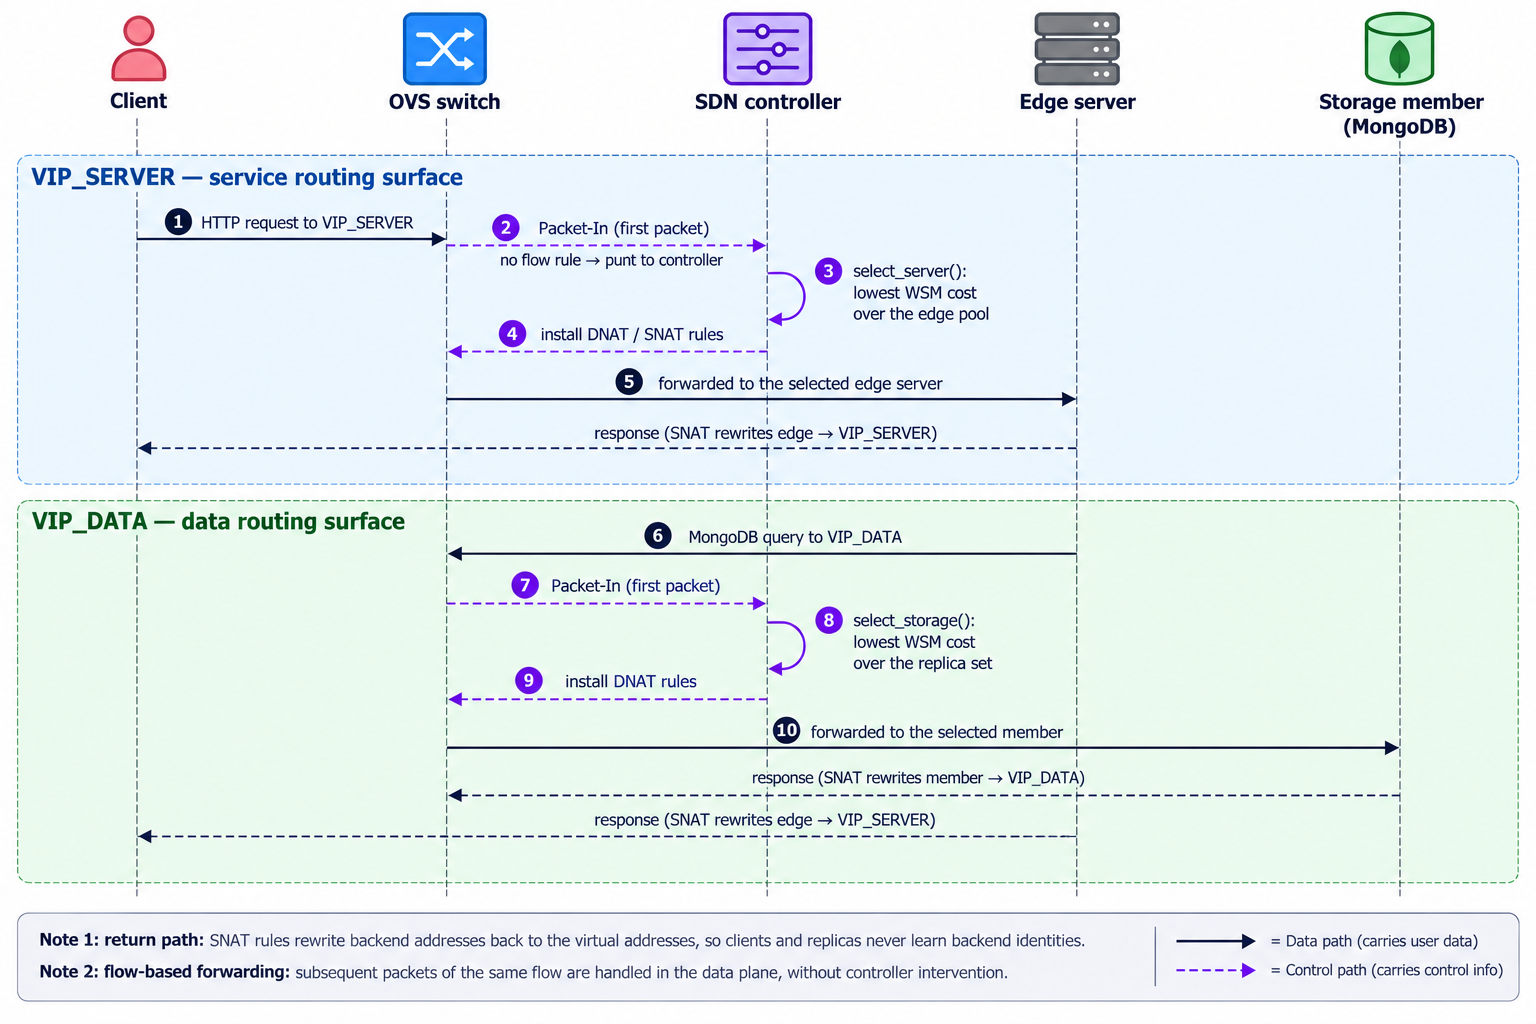
\includegraphics[width=0.9\textwidth]{images/vip_routing_sequence.png}
    \caption{Double-VIP routing sequence: a client request addressed to
    \texttt{VIP\_SERVER} triggers backend selection in the controller, and
    the edge server's storage access through \texttt{VIP\_DATA} triggers the
    selection of a replica-set member.}
    \label{fig:vip_routing_sequence}
\end{figure}

\subsection{Control and Observation Paths}
Edge servers and storage components emit resource and request observations to
their local telemetry aggregator through \ac{ZMQ}. Each aggregator forms
windowed summaries that are consumed by the controller. These summaries inform
both backend selection and elasticity decisions, while topology exchange
maintains awareness of peer-domain resources. The aggregation-to-controller
link is the configurable telemetry-delivery interface.

\begin{figure}[H]
    \centering
    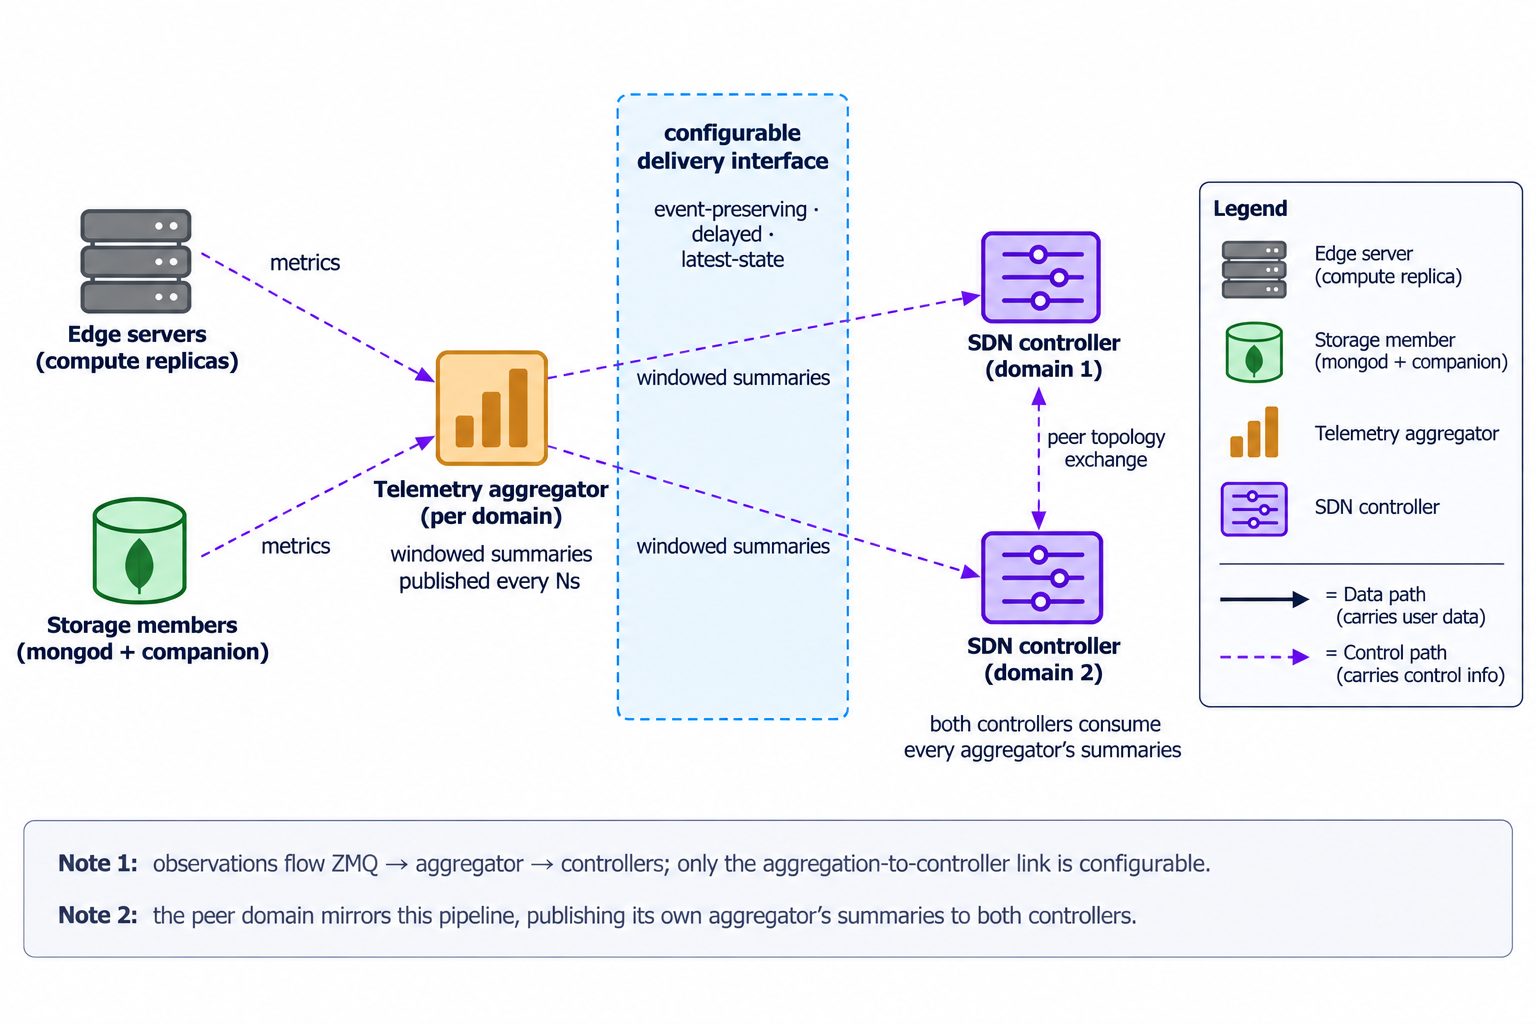
\includegraphics[width=0.9\textwidth]{images/telemetry_delivery_paths.png}
    \caption{Control and observation paths: edge servers and storage members
    publish observations to the per-domain telemetry aggregator, whose
    windowed summaries reach both peer controllers through a configurable
    delivery interface.}
    \label{fig:telemetry_delivery_paths}
\end{figure}

    The architecture therefore separates the request data path, the telemetry
observation path, and the slow infrastructure-management path while retaining
their coordination within each domain's controller process. The concrete
implementation of these paths is described in Chapter~4.

    The deployment evaluated in this dissertation runs the two domains on a
single host, with an emulated wide-area link; no performance claim is made
for a real geo-distributed wide-area deployment. The testbed is described
in the experimental setup of Chapter~5.

\section{Distributed Elastic Allocation of Resources}\label{sec:elastic_allocation}
The platform scales capacity along two axes: edge-service replicas, which
serve requests, and storage members, which hold the service state. Each axis
has its own observation signal, its own action, and its own admission and
release procedure, so that pressure on the service tier and pressure on the
data tier can be addressed without conflating the two. The two axes are
described in turn.

\subsection{Scaling Policy}\label{sec:scaling_policy}
The policy is instantiated once per resource tier, with tier-specific
signals and parameters. Each tier is observed through two signals: a
utilisation signal and a latency signal. For each telemetry window $w$, let
$c(w)$ denote the window's utilisation and $t(w)$ its typical latency. Each
signal is first mapped onto the unit interval: a value at or below its floor
contributes nothing, a value at or above the floor plus its span contributes
the maximum, and intermediate values contribute proportionally, so that a
single extreme window cannot dominate the score. The two normalised
components are combined with weights $w_{\mathrm{util}}$ and
$w_{\mathrm{lat}}$ into the degradation score
\begin{equation}
\begin{split}
    s(w) &= \frac{w_{\mathrm{util}}\,\hat{c}(w) + w_{\mathrm{lat}}\,\hat{t}(w)}
                 {w_{\mathrm{util}} + w_{\mathrm{lat}}}, \\
    \hat{c}(w) &= \min\left(1,\ \max\left(0,\ \frac{c(w)-c_0}{c_\Delta}\right)\right), \\
    \hat{t}(w) &= \min\left(1,\ \max\left(0,\ \frac{t(w)-t_0}{t_\Delta}\right)\right),
\end{split}
\end{equation}
which therefore always lies between zero and one, where:
\begin{itemize}[leftmargin=*, itemsep=0pt]
    \item $c(w)$ -- utilisation of the scored tier observed in window $w$;
    \item $t(w)$ -- typical latency of the scored tier observed in window $w$;
    \item $c_0$, $t_0$ -- signal floors: at or below these values a signal contributes nothing;
    \item $c_\Delta$, $t_\Delta$ -- signal spans: at or above floor plus span a signal contributes the maximum;
    \item $\hat{c}(w)$, $\hat{t}(w)$ -- normalised components of window $w$, each in $[0,1]$;
    \item $w_{\mathrm{util}}$, $w_{\mathrm{lat}}$ -- configurable weights of the utilisation and latency components.
\end{itemize}
    The floors, spans, and weights are configuration parameters, set
independently for each tier: for the service tier the signals are CPU
utilisation and request-processing latency, while for the data tier they
are storage utilisation and data-access latency.

    A window is considered degraded when its score reaches an adaptive
threshold, and a scale-up is requested only when degradation is sustained
across a required number of recent windows. Let $\mathcal{W}_n$ be the set
of the last $W$ windows and $R$ the required number of degraded windows;
the scale-up condition is
\begin{equation}
\begin{split}
    \left|\,\{\, w \in \mathcal{W}_n : s(w) \geq \theta(k) \,\}\right| &\geq R, \\
    \theta(k) &= \min\big(\theta_{\mathrm{base}} + k\,\Delta\theta + \beta_{\mathrm{peer}},\ \theta_{\max}\big),
\end{split}
\end{equation}
where:
\begin{itemize}[leftmargin=*, itemsep=0pt]
    \item $\mathcal{W}_n$ -- sliding set of the most recent $W$ windows;
    \item $R$ -- minimum number of degraded windows required to request a scale-up;
    \item $k$ -- number of dynamic units currently in the tier's pool;
    \item $\theta(k)$ -- adaptive degradation threshold with $k$ dynamic units in the pool;
    \item $\theta_{\mathrm{base}}$ -- base threshold;
    \item $\Delta\theta$ -- threshold increment per additional dynamic unit;
    \item $\theta_{\max}$ -- upper bound of the adaptive threshold;
    \item $\beta_{\mathrm{peer}}$ -- addend applied while the peer domain is healthy enough to absorb spillover traffic.
\end{itemize}
    The threshold $\theta(k)$ adapts upward as capacity grows, so each
additional unit faces a higher bar, bounded by $\theta_{\max}$, and
$\beta_{\mathrm{peer}}$ raises it slightly while the peer domain is healthy
enough to absorb spillover traffic. A cooldown after each action and a
per-tier cap on the number of units keep the number of scale actions
bounded.

    A window is declared idle when both signals fall below their idle
thresholds,
\begin{equation}
    c(w) < \tau_c \quad\text{and}\quad t(w) < \tau_t,
\end{equation}
where:
\begin{itemize}[leftmargin=*, itemsep=0pt]
    \item $\tau_c$, $\tau_t$ -- idle thresholds of the utilisation and latency signals;
    \item $R_\downarrow$, $W_\downarrow$ -- required idle windows and window size of the scale-down rule.
\end{itemize}
    A scale-down is requested only when idleness is sustained across
$R_\downarrow$ of the last $W_\downarrow$ windows, a sliding window longer
than the scale-up one, which prevents a transient data-bound stall from
being misread as idle capacity. The concrete parameter values used in the
evaluation are reported in the experimental setup of Chapter~5.

\subsection{Services}\label{sec:elastic_compute}
Service capacity is a per-domain pool of containerised edge servers, each
capable of serving any request addressed to the domain's virtual service
address. All storage access performed by a service replica goes through the
domain's virtual data address, so a replica carries no physical knowledge of
the storage tier. Service scale-up applies the policy defined
in \ref{sec:scaling_policy}, with CPU utilisation
and request-processing latency as signals.

    A newly provisioned service replica is recorded through an explicit
registration step; the replica becomes eligible for backend selection only
once it is visible in the routing pool used by the selector. The point at
which registration occurs relative to application readiness is itself a
configurable design dimension: the replica may be admitted immediately upon
creation, or admission may be deferred until a readiness condition is
verified, which is the mechanism examined for the admission interface of
the demand-to-capacity chain.

    Service scale-down removes the least disruptive eligible replica, applying
the idle predicate defined in \ref{sec:scaling_policy}. Removal proceeds in
two phases: the replica is first withdrawn from the routing pool and
signalled to finish its in-flight requests, and only after it drains is its
network attachment removed. A pending drain can be cancelled if load
rebounds before the replica exits, favouring fast recovery over aggressive
reclamation.

\subsection{Data}\label{sec:elastic_data}
The replica set is the unit in which storage capacity is scaled. The data
tier of each domain runs as a MongoDB replica set whose primary serves the
clients' writes and whose secondaries replicate the data and absorb the
remainder of the traffic. Storage scale-up is a membership change: the
controller provisions a new storage member, joins it to the set, and admits
it to the data path only once the member has reached the state at which it
can serve reads, so that traffic is never directed to a member that cannot
yet serve it. The preparation may also be decoupled from the reaction: a
ready member can be held in reserve outside the routing pool and activated
when a data action fires, removing the initial readiness wait from the
reaction path, with a new reserve prepared immediately afterwards.

    Storage scale-down removes an idle member while the remaining members keep
serving. Only members added by the platform are eligible for removal, so the
set's original membership is never disturbed, and the decision applies the
idle predicate defined in \ref{sec:scaling_policy} with the data tier's
utilisation and latency signals, evaluated over sustained low data-access
latency and utilisation.

    Beyond the membership change, the platform defines three data-placement
tiers, named here for completeness: Tier 0, direct remote reads over the
virtual data path; Tier 1, a partial hot copy held in the consumer domain;
and Tier 2, the replica-set extension described above. These locality
mechanisms are platform capabilities rather than evaluated treatments: they
are disabled or held constant wherever an evaluation requires their
isolation, and the capacity action evaluated in this dissertation is the
same-domain membership change.

\section{Monitoring and Decision Engine}\label{sec:monitoring_decision}
Observation begins at the producers. Each service replica emits a
per-request record of its resource state and request experience, and each
storage member's companion process emits periodic replication and resource
state. A per-domain aggregator collects these records and publishes a
windowed summary at a fixed cadence, so that time is observed as a regular
sequence of windows and every window, including idle ones, carries an
evaluation outcome.

    The delivery of these summaries to the controller is an explicit, configurable
interface. The default delivery pushes each completed window as it is
published. Alternative delivery modes supply the same windowed evidence in
other forms, such as periodic retrieval of only the most recent window or
ordered replay of a retained window history, so that the effect of delayed
or incomplete demand evidence can be studied while the aggregation, the
workload, and the decisions remain identical.

    Inside the controller, the summaries feed two consumers. The first is the
routing state: per-backend metrics update the state that backend selection
uses. The second is the decision engine: per-domain degradation scores,
computed per resource tier from bounded utilisation and typical request
latency, are evaluated against adaptive thresholds over sliding windows.
When a tier's predicate is sustained, the decision engine emits a typed,
prioritised request for a capacity action, with data-side actions given
precedence over service-side actions. Scale-down requests arise from
separate idle predicates. 

    The decision engine may also be configured to commit to a single action per
window when several tiers signal simultaneously, which is the selection
interface of the demand-to-capacity chain. Lifecycle signals, such as the
completion of a drain or the readiness of a storage member, reach the same
decision path as control events, so that admission and release follow the
same disciplined flow as the actions themselves.

\section{Control Workflow}\label{sec:control_workflow}
The control workflow separates three execution contexts that share one
process but never share blocking: the packet context, which handles flow
decisions and never waits on slow work; the observation context, which
evaluates telemetry windows and emits action requests; and the action
context, which performs infrastructure mutations such as provisioning,
drain, and removal.

    The workflow traverses the demand-to-capacity chain introduced in
\ref{sec:context_motivation}. A change in demand alters the request
experience reported by the service replicas; the window that contains that
change is published and delivered; the decision engine evaluates it and, if
the tier predicate is sustained, emits an action request; the action context
executes it; the provisioned unit reaches its readiness state and is
admitted to the corresponding routing pool; and from the next packet the
data plane can direct traffic to it, which completes the chain when the new
unit serves its first successful request. Each step of this chain is
instrumented, so the timeline from demand observation to usable capacity is
recorded end to end.

    State crosses these contexts through shared structures rather than through
direct calls. The observation context writes the telemetry state and the
action requests; the routing pools are updated as units are provisioned,
readied, and removed; and the packet context reads both on each flow
decision.
Because the packet context is never blocked by the action context, a
long-running mutation cannot stall request steering, and because the action
requests are queued and prioritised, detection is never blocked by
execution.

    Across domains, the peer controllers exchange topology state so that each
controller is aware of the peer domain's resources, while acting on its own
domain's demand. The concrete realisation of this design, the technologies
that implement each context, and the validation of the resulting platform
are the subject of Chapter~\ref{ch:implementation}; the experimental
characterisation of the three interfaces is presented in
Chapter~\ref{ch:results}.


\chapter{Implementation of Proposed Solution}\label{ch:implementation}

\section{Experimental infraestructure}\label{sec:impl_infraestructure}
% TODO: two emulated domains on a single cloud-VM host; Docker containers;
% OVS topology (two LANs + WAN bridge, tc-netem); WAN emulation profiles.

\section{Distributed Elastic Allocation of Resources}\label{sec:impl_elastic}

\subsection{Services}\label{sec:impl_compute}
% TODO: Edge server (Python/Flask); container lifecycle (build, start, health check,
% OVS wiring, drain, removal); VIP_SERVER registration. BACKEND_SELECTION_POLICY
% env var (topology_host / topology_slowstart / topology_lifecycle) = RQ3 propagation
% mechanism; requires a compute readiness probe + pending-backend registry (thesis_overview.md §6-RQ3).

\subsection{Data}\label{sec:impl_data}
% TODO: MongoDB replica sets; programmatic rs.add()/rs.remove(); VIP_DATA routing;
% epoch recovery; retryReads; connection pooling; storage container lifecycle.
% Conntrack-based routing for VIP_DATA.

\section{Monitoring and Decision Engine}\label{sec:impl_monitoring}
% TODO: Aggregator (ZMQ PUB/SUB + HTTP cache); collect_resource_stats.py
% (domain + debug + per-node CSVs); telemetry source abstraction
% (ZmqTelemetrySource, PollingTelemetrySource). Degradation score with
% configurable weights via SCALEUP_W_CPU / SCALEUP_W_T_PROC env vars;
% ElasticityManager. RQ2 requires a bottleneck-classification gate that logs episode label,
% evidence, selected/rejected action, and action budget (thesis_overview.md §6-RQ2).

\section{Control Workflow}\label{sec:impl_control}
% TODO: OS-Ken/Ryu controller; 3 greenthreads; shared data structures;
% key algorithm pseudo-code (degradation score → threshold → sliding window →
% alert → spawn); Double-VIP ARP interception + DNAT/SNAT.

\section{Implementation Validation}\label{sec:impl_validation}
% TODO: Golden-config stability experiments (15+ runs, variance ≤0.23%);
% mechanism validation (Tier 2, Tier 1, compute, conntrack);
% algorithm correctness via stable behavior, not code inspection.



\chapter{Experimental Results}\label{ch:results}
% Section order follows the demand-to-capacity chain: RQ1 → RQ2 → RQ3 → Synthesis.

\section{Experimental Setup}\label{sec:experimental_setup}
% TODO: emulated two-domain testbed on a single host; no real geo-distributed
% WAN claims (C1); one table per RQ (treatment, held constants, workload,
% experimental unit, replication, exclusions, statistical test); do NOT claim
% a common nine-phase workload across RQs.
% TODO (absorbed from the removed Evaluation Methodology chapter §5.2–§5.3):
% within-system, single-variable manipulation; baselines encode architectural
% properties, not competing products; each RQ holds the other two interfaces
% constant; demand model / 9-phase workload (thesis_overview.md §2). Metrics:
% reaction latency (time from demand shift → usable capacity, segmented per RQ);
% service quality (p50/p95/p99 latency, failure rate, offered vs completed requests);
% control overhead (CPU%, RSS). Per-RQ outcomes: RQ1 — completed/missed windows,
% info age, delivery delay; RQ2 — time to recover bottleneck-specific pressure,
% node-minutes, action relief; RQ3 — ready→admitted, admitted→first-flow,
% first-flow→first-success, useful initial request share, where "admitted" =
% visible in the selector's actual eligible pool (or first flow installed), not
% merely a registration/role-membership update. Per-RQ locks: RQ1 holds
% scaling+routing policy fixed; RQ2 holds telemetry delivery+routing fixed; RQ3
% holds telemetry delivery+selection fixed (thesis_overview.md §6).

\section{Telemetry Delivery Semantics (RQ1)}\label{sec:results_rq1_delivery}
% TODO (RQ1): completed/missed overload windows; information age and delivery delay; time from
% demand shift → scaling decision and → usable capacity; offered/completed requests; latency
% distributions and failure rate; controller/telemetry overhead. Compare event-preserving vs
% delayed event-preserving vs latest-state delivery (thesis_overview.md §6-RQ1).

\section{Bottleneck-Aware Scaling Action (RQ2)}\label{sec:results_rq2_action}
% TODO (RQ2): time to recover bottleneck-specific pressure; time to usable capacity; p50/p95/p99
% latency; failures and completed offered demand; compute and storage node-minutes; number of
% scale actions; relief in the targeted tier. Structure follows matched vs mismatched selection:
% aligned cells (cf_cb/ba_cb, sf_db) validate the mechanism; mismatched cells (sf_cb, cf_db)
% quantify the wrong-action cost; the ba cells report the classifier's decision trace as a
% covariate, not an assumption (thesis_overview.md §6-RQ2; v3 results: wrong-action service cost
% small at the tested intensity, resource waste and tail-latency noise carry the signal).

\section{Readiness Admission to Traffic (RQ3)}\label{sec:results_rq3_readiness}
% TODO (RQ3): backend-ready → routing-admitted delay (admitted = selector-visible pool
% inclusion); admitted → first-flow delay; first-flow →
% first-successful-response delay; useful initial request share; transition-window latency and
% failures; time from scale decision to usable capacity. Direct lifecycle notification vs periodic
% discovery, selection function held fixed (thesis_overview.md §6-RQ3). Supporting calibration
% evidence: old RQ2 slowstart ≈ periodic discovery, ~31 s idle-capacity penalty (n=9).

\section{Network Performance}\label{sec:results_network}
% TODO: Control-plane overhead (CPU%, RSS); cross-LAN latency;
% WAN emulation effects; telemetry delivery overhead.

\section{Scalability Analysis}\label{sec:results_scalability}
% TODO: Behavior under increasing load; scaling outcome description
% (breached windows vs. spawns completed); mechanism activation patterns.
% Resource allocation efficiency: does the system deploy resources only when
% justified? Storage and compute node counts across phases.

\section{Discussion: Synthesis Across Interfaces}\label{sec:discussion}
% TODO: synthesize per-interface effects (RQ1/RQ2/RQ3) measured under a common workload, resource
% configuration, and event schema. Which interface matters most under which conditions? Sharpest
% trade-offs? What is negligible? Implications for stateful edge-service designers.
% Data-placement strategies (Tier 0/1/2) remain held-constant platform context; experimental
% characterization of data-locality trade-offs is deferred to future work.



\chapter{Conclusions and Future Work}\label{ch:conclusions}

\section{Conclusions}\label{sec:conclusions}
% TODO: Summary of findings across RQ1, RQ2, RQ3.

\section{Research Contributions}\label{sec:contributions_revisited}
% TODO: Restate the four contributions with evidence from results.

\section{Limitations}\label{sec:limitations}
% TODO: Controlled testbed; emulated (not real) WAN; single host; single window size;
% statistical power (n=3 per condition); RQ1/RQ2/RQ3 rely on required extensions and are
% designed, not fully measured (thesis_overview.md §6); the old RQ2 slowstart result (~31 s,
% n=9) is supporting calibration evidence for RQ3's periodic-discovery condition, not final
% evidence; MongoDB-specific mechanisms (Double-VIP); no end-to-end coordination penalty is
% claimed — per-interface results are synthesized only under a matched schema.

\section{Future Research Directions}\label{sec:future_work}
% TODO: Compound coordination delay injection experiment (emulate full separation
% with configurable delays at both handoff points simultaneously); window size
% variation (freshness vs. noise trade-off); Tier 1 Selective Sync full implementation
% and experimental validation; data locality experimental characterization (Tier 0 vs.
% Tier 1 vs. Tier 2 cold vs. Tier 2 warm — designed, deferred from RQ3 scope);
% larger-scale deployment; real-world traces; ML-driven threshold adaptation.

\end{document}
% =====================================================================